\documentclass[font=12pt]{article}
\usepackage{../hdr}
\usepackage{graphics, graphicx,subcaption}
\newcommand{\mycourse}{02-510 Computational genomics}

\begin{document}

\medskip
\setcounter{section}{1}
\section{Sequence Alignment}

\newpage
\section{Short read assembly}

\newpage
\section{Sequencing}

\newpage
\section{Normalization}
\subsection*{Assumption}
Assume the subset of the genes in the sample are expressed at the same total level across all cells / samples
\subsection{Methods}
\begin{itemize}
	\item \textbf{\textcolor{red}{RPKM} - read per kilobase of transcript per million reads of library}
	\begin{itemize}
		\item Corrects for coverage, gene length
		\item 1 RPKM ~ 0.3 -1 transcript / cell
		\item Comparable between different genes within the same dataset
		\item packages: TopHat / Cufflinks
		\[ RPKM = \frac{\text{no. of reads mapped to gene G} \cdot 10^9 }{\text{total no. of mapped reads} \cdot \text{length of gene G}}\]
	\end{itemize}
	\item \textbf{\kyw{FPKM} - fragments Per Kilobase of exon model per Million mapped fragments}
	\begin{itemize}
		\item similar to FPKM
		\item for pair-end seq, $ FPKM = 2 RPKM $
		\[ FPKM = \frac{\text{no. of fragments mapped to the exons} \cdot 10^9 }{\text{total no. of mapped reads} \cdot \text{length of the exon}}\]
	\end{itemize}
	\item \textbf{\kyw{TPM} - transcript per million}
	\begin{itemize}
		\item Normalizes to transcript copies instead of reads 
		\item Longer transcripts have more reads
		\item RSEM, HTSeq
		\item steps:
	\end{itemize}
	\begin{enumerate}
		\item $ RPK = \dfrac{\text{read count of gene}}{\text{length of gene}} $
		\item $ \text{scaling factor} = \sum RPK / 10^6 $
		\item $ TPM = \dfrac{RPK}{\text{scalling factor}} $
	\end{enumerate}
	\item additional assumptions
	\begin{enumerate}
		\item values are exactly the same between runs (genes could have variable values)\\
		$\to$ quantile normalization
		\item values are normally distributed w same mean and var across samples\\
		$\to$ scale factor normalization
		\item assume some genes have stable values over runs (rank invariant)\\
		$\to$ invariant set normalization
	\end{enumerate}
	\item \textbf{\kyw{TMM} - Trim Mean of M}
	\begin{itemize}
		\item high level idea: remove extreme values before normalizing
		\item intuition:\\
		sample A and B both have 100 genes sequenced to the same depth, 90 genes in A and B are expressed at about the same level, last 10 genes expressed at extremely high level in B\\
		$\to$ could appear as the first 90 genes expressed twice as high in A than in B, which does not make sense\\
		Reason: fixed amount of sequencing real estate
		\item observed coutns of gene g in experiment k: $ E[Y_{g,k}] = \dfrac{\mu_{g,k} L_g}{S_k} N_k $, where
		\begin{itemize}
			\item $ S_k = \sum_g \mu_{g,k}L_g $
			\item $ \mu_{g,k} $ true expression level of gene g in experiment k
			\item $ L_g $ length of gene g
			\item $ N_k $ total no. of reads for experiment k
		\end{itemize}
		\item $ M_g = \log \dfrac{Y_{g,k}/N_k}{Y_{g,k'}/N_{k'}} $
		\item $ A_g =  \log Y_{g,k}/N_k + \log Y_{g,k'}/N_{k'}$
		\item trim off genes with extreme M and A values (in the paper, took 5\% and 30\% as cutoff)
		\item compute ratio based on all other genes
	\end{itemize}
\end{itemize}
\subsection{Transformation}
\begin{itemize}
	\item While ratios are useful, not symmetric\\
	$\to$ hard to visualize different changes
	\item use a log transform, and focus on the log ratio
	\[y_i = \log \dfrac{R_i}{G_i}\]
	\item Empirical studies have also shown that in microarray experiments the log ratio of (most) genes tends to be normally distributed
\end{itemize}


\newpage
\section{DE gene}
\subsection{Problem}
\begin{itemize}
	\item log-fold change isn't ideal (there are problems)
	\item noise from technology too
	\item expression being double the amount $\to$ how reliable? $\to$ variation estimation
	\item easy to estimation variation if large biological models, but often only 2-3 replicate available
	\item Solution: often assume some mathematical model
\end{itemize}
\subsection{Statistical models}
\begin{itemize}
	\item Gaussian
	\begin{itemize}
		\item mean $ \mu $, var $ \sigma^2 $
	\end{itemize}
\end{itemize}
A couple methods based on counts...
\begin{itemize}
	\item Binomial
	\begin{itemize}
		\item \[P(x=k)= {n\choose k} p^k (1-p)^{n-k} \]
		\item mean: $ np $, var: $ np(1-p) $
	\end{itemize}
	\item Poisson
	\begin{itemize}
		\item \[P(x=k) = \dfrac{\lambda^k e^{-\lambda}}{k!}\]
		\item mean = var = $ \lambda $
	\end{itemize}
	\item Negative Binomial
	\begin{itemize}
		\item common when data has variance $ >> $ mean (overdispersed)
		\item defined as the number of successed in a seq of Bernoulli trials before \cmt{some number of} event $ r $ occurs, eg. no. of trials until 3 heads
		\item Thus appropriate for modelling biological replicates
		\item \[P(x=n) = {n-1\choose k}p^k(1-p)^r\]
		where $ r $: no. of failures, $ k $: no. of successes until $ r $ failures, and $ n = k + r $
		\item mean: $ rp/(1-p) $, var = $ rp / (1-p)^2 $
		\item \underline{can be re-written in a format similar to Poisson dist.}
		\item Poisson assumes same mean and variance, whereas NB assumes larger variance
		\item $\to$ \kyw{dispersion parameter $ \alpha $} s.t. 
		\[\text{mean} = \lambda, \text{ var} = \lambda + \alpha\lambda^2\]
		\item NB = Poisson when $ \alpha = 0 $
	\end{itemize}
\end{itemize}
\subsection{Hypothesis testing}
\begin{itemize}
	\item $ H_0 $: mean expression of the gene under two conditions are the same
	\item p-value: how likely it is to see the data we observe under $ H_0 $
	\item eg. one sample $ t $ test, two sample $ t $ test, non-parametric rank test, \textbf{$\chi^2$ test}
\end{itemize}
\subsection{log-likelihood ratio test}
\begin{itemize}
	\item Compute the likelihood under $ H_0 $ and $ H_1 $. ie. $$ \Pi_{i\in A} P(x=i | \text{model param}) \Pi_{i\in B} P(x=i | \text{model param}) $$
	\item log-likelihood ratio = $ \log\dfrac{L1}{L0} $ (note we are assuming equal variance under both hypothesis)
	\item degree of freedom: no. of free parameters - 1
\end{itemize}
\subsection{limitations}
\begin{itemize}
	\item assume specific probabilistic model
	\item need many replicates
	\item multiple hypothesis testing issue
\end{itemize}
\subsection{Multiple hypothesis testing}
\begin{itemize}
	\item eg. 1 trillion monkeys, one of the randomly typed out shakespear
	\item Bonferroni Correction
	\begin{itemize}
		\item very conservative
		\item may cause us to miss out genes
		\item adjusted p-val = original pval / no. of genes testing
	\end{itemize}
	\item FDR
	\begin{itemize}
		\item 100 genes identified w p-val 0.05, then 5 genes are probably falsely discovered
		\item \kyw{more stuff from hw2???}
	\end{itemize}
	\item Permutation based methods
	\begin{itemize}
		\item idea is to determine the prob. of seeing the real data in a random sample
		\item divide by no. of permutations done
		\item can be a problem when the no. of samples small
	\end{itemize}
	\item time series data are often too hard to be considered, not always possible
\end{itemize}
\newpage
\section{Clustering}
\subsection{Motivations}
\begin{itemize}
	\item clustering genes $\rightarrow$ 
	\item clustering cells $\rightarrow$
	\item clustering both
	\item \textcolor{blue}{distance measure:} (dissimilarity) $\in\mathbb{R}$
		\begin{itemize}
			\item eg. euclidian dist, 1-correlation coefficient
		\end{itemize}
\end{itemize}
\subsection{hierarchical clustering}

\subsection{Partitional clustering}
\begin{itemize}
	\item non-hierarchical, each instance is placed in exactly one of k non-overlapping clusters
	\item eg. k-means
\end{itemize}

\subsubsection{Gaussian mixture models}
\begin{itemize}
	\item the importance of initialization
\end{itemize}
\subsection{Graph based clustering}

\subsection{Cross-validation}
\subsubsection{internal validation}
\subsubsection{external validation}
\subsubsection{hypergeometric distribution}

\subsection{Bi-clustering}
find subsets of genes 

\newpage
\section{Classification}
\subsection{Types of classifiers}

\subsection{Weighted voting}

\subsection{Bayes classifier}

\subsection{Naive Bayes classifiers}

\subsection{Feature selection}

\subsection{SVM}

\subsection{Challenges in computational analysis of omics data for development of molecular signatures}
\begin{itemize}
	\item ez to develop predictive model $\to$ easy to believe a model is good when it's not
	\item several theoretical/practical problems exist
	\item most cannot be validated on an independent cohort, unfortunately :/
\end{itemize}

\newpage
\section{Single Cell}
Goals:
\begin{enumerate}
	\item cells differentiates into sub-celltypes
	\item unknown celltype discovery
\end{enumerate}

\subsection{Dimensionality reduction}
Motivation:
\begin{enumerate}
	\item high dim data often has lower dim representation w/o much reconstruction error
	\item lower dim representation can often represent info about high dim pairwise dist.
\end{enumerate}
Types of dim-red:
\begin{itemize}
	\item \textcolor{red}{Global methods}
		\begin{enumerate}
			\item all pairwise dist equally impt
			\item lower dim pairwise dist fit high-dim ones
			\item often use magnitude or rank order
		\end{enumerate}
	\item \textcolor{red}{Local methods}
		\begin{enumerate}
			\item only local dist reliable in high dim
			\item more weight on modelling local dist correctly
		\end{enumerate}
\end{itemize}
Methods:
\begin{itemize}
	\item PCA
		\begin{itemize}
			\item finds directions with largest variance
			\item minimize squared reconstruction error
			\item equiv to liner autoencoders
			\item Steps of PCA
			\begin{enumerate}
				\item $\overline{X}$: mean of all samples(usually rows), adjust $ X \rightarrow X' = X - \overline{X}$ 
				\item covar matrix $ C = X'^T X'$
				\item find eigenvectors and eigenvalues of $C$, ie. all pair of $\vec{v}, \lambda$ st. $ C\vec{v} = \lambda \vec{v}$
				\item eigenvalues can be used to calculate percentage of total variance for each component \[v_j = 100\frac{\lambda_j}{total \quad eigenvalue}\] 
			\end{enumerate}
		\end{itemize}
		\textcolor{blue}{This is non-parametric method, do not insist on a parametric encoding function}
	\item Multi-Dimensional Scaling
		\begin{itemize}
			\item  arrange low dim points to minimize diff between pairwise distances in the high and low D space
			\item a possible approach: start w a random vector, perform gradient decent
			\item \textcolor{red}{is there something to do with PCA?} then we don't need iterative method
		\end{itemize}
	\item Sammon (non-linear autoencoder)
		\begin{itemize}
			\item  with extra layers, much more powerful than PCA, but can be slow to converge, and can get stuck on local optima
			\item Multi-Dimensional Scaling(MDS) can be made non-linear by giving higher weights to smaller distances, a popular formula is 
				\[ cost = \sum_{ij} \left(\frac{|x_i - x_j| - |y_{i}-y_j|}{|x_i - x_j|}\right)^2\]
				where $ x$ is high-dim dist, and  $y$ is low-dim dist
			\item still slow and get stuck on local optima
		\end{itemize}
\end{itemize}

\subsection{Graph-basd method}
		\begin{itemize}
			\item address uniform circularity
			\item  \textcolor{red}{Isomap} is a dim-red technique based on graphs
				\begin{itemize}
					
			\item each datapoint is connected to $k$ nearest neighbor in high-dim
			\item edge weights = euclidean dist
			\item approx of distance = shortest path in contracted graph
			\end{itemize}
		\item \textcolor{red}{Probabilistic local MDS}
			\begin{itemize}
				\item local distances are more impt than non-local ones
				\item in this way all local distances are given equal importance	\end{itemize}

		\item \textcolor{red}{stochastic neighbor embedding(SNE)} has a probabilistic way to decide if a distance is local
			\begin{itemize}
				\item convert global distances into probability of one datapoint picking another datapoint as its neighbor \textcolor{blue}{(what defines a neighbor tho) - still about isomaps?}
				\item each point in high-dim has a conditional probability of picking any other point as its neighbor
			\item distribution (some sort of Gaussian) is over high-dim distances (if high-dim coords unavailable, a similarity / dissimilarity matrix may be used)\\ $p_{j|i}$ is the prob. of picking j given starting at i in high-dim.
				\[ P_{j|i} = \frac{e^{-2d_{ij}^2 / 2\sigma_i^2}}{\sum_k e^{{-d_{ik}^2}/{2\sigma_i^2}}} \]
				\item having the probabilities potentially allow us to throw away the raw high-dimensional data
				\item evaluation done using pairwise distance in low dimensional map (shows how well the lower dim representation models high-dim data ig)\\
					$q_{j|i}$ is the prob of picking j given starting at i in low-dim
				\item compute the \textcolor{red}{Kullback-Leibler divergence} between prob. in the high-dim and low-dim spaces \textcolor{blue}{(why not just use dist in high dim?) - more space / time efficient}
				\item nearby pts in high-dim should be close in low-dim
			\end{itemize}
		\item picking $\sigma$ used to compute  $p$ - the radius of the gaussian
			 \begin{itemize}
				 \item different radius is needed in different parts of the space to keep the no. of neighbors constant
				 \item big radius $\rightarrow$ high entropy for distribution over i's neighbors
				 \item small radius $\rightarrow$ low entropy
				
			\end{itemize}
		\item \textcolor{red}{Symmetric SNE}
			\begin{itemize}
				\item simpler than stochastic
				\item works best if different procedures are used for computing $p$'s and  $q$'s.
				\item compromise: no longer guarantees that if using same dimension will produce optimal solution
				\item turn conditional prob into symmetric pairwise probabilities
			\end{itemize}
		\item Optimization methods for SNE
			\begin{itemize}
				\item simulated annealing could lead to better global optimization
				\item add Gaussian noise to $y$ location in each update
				\item spend longer time at noise level where global structure start to form
				\item \textcolor{red}{t-SNE} - use Gaussian at many (infinite) spatial scales, cheaper as we don't have to exponentiate anymore \textcolor{blue}{(why????)} 
			\end{itemize}
				\end{itemize}
\subsection{Supervised dim-red: Neural networks}
\begin{itemize}
	\item last few layers have much fewer values than inputs
	\item use intermediate layers as lower-dim representations
	\item can easily add prior biological knowledge, such as protein interactions or transcription factors
	\item essentially, some nodes in the hidden layer are same as before, others are based on biological info
\end{itemize}
\subsubsection{Additional NN architecture: Siamese}
\begin{itemize}
	\item supervised, but not trying to maximize training accuracy
	\item input: whether each pair is similar
	\item output: binary label of similar / not similar
	\item thus directly optimize dim-red layer for KNN
\end{itemize}
\newpage
\section{ChIP-Seq}
\subsection{Background}
\begin{itemize}
	\item transcription factors bind to specific locations on the chromosome
	\item the binding is highly specific
	\item this has impact on gene regulation
	\begin{figure}[h!]
		\centering
		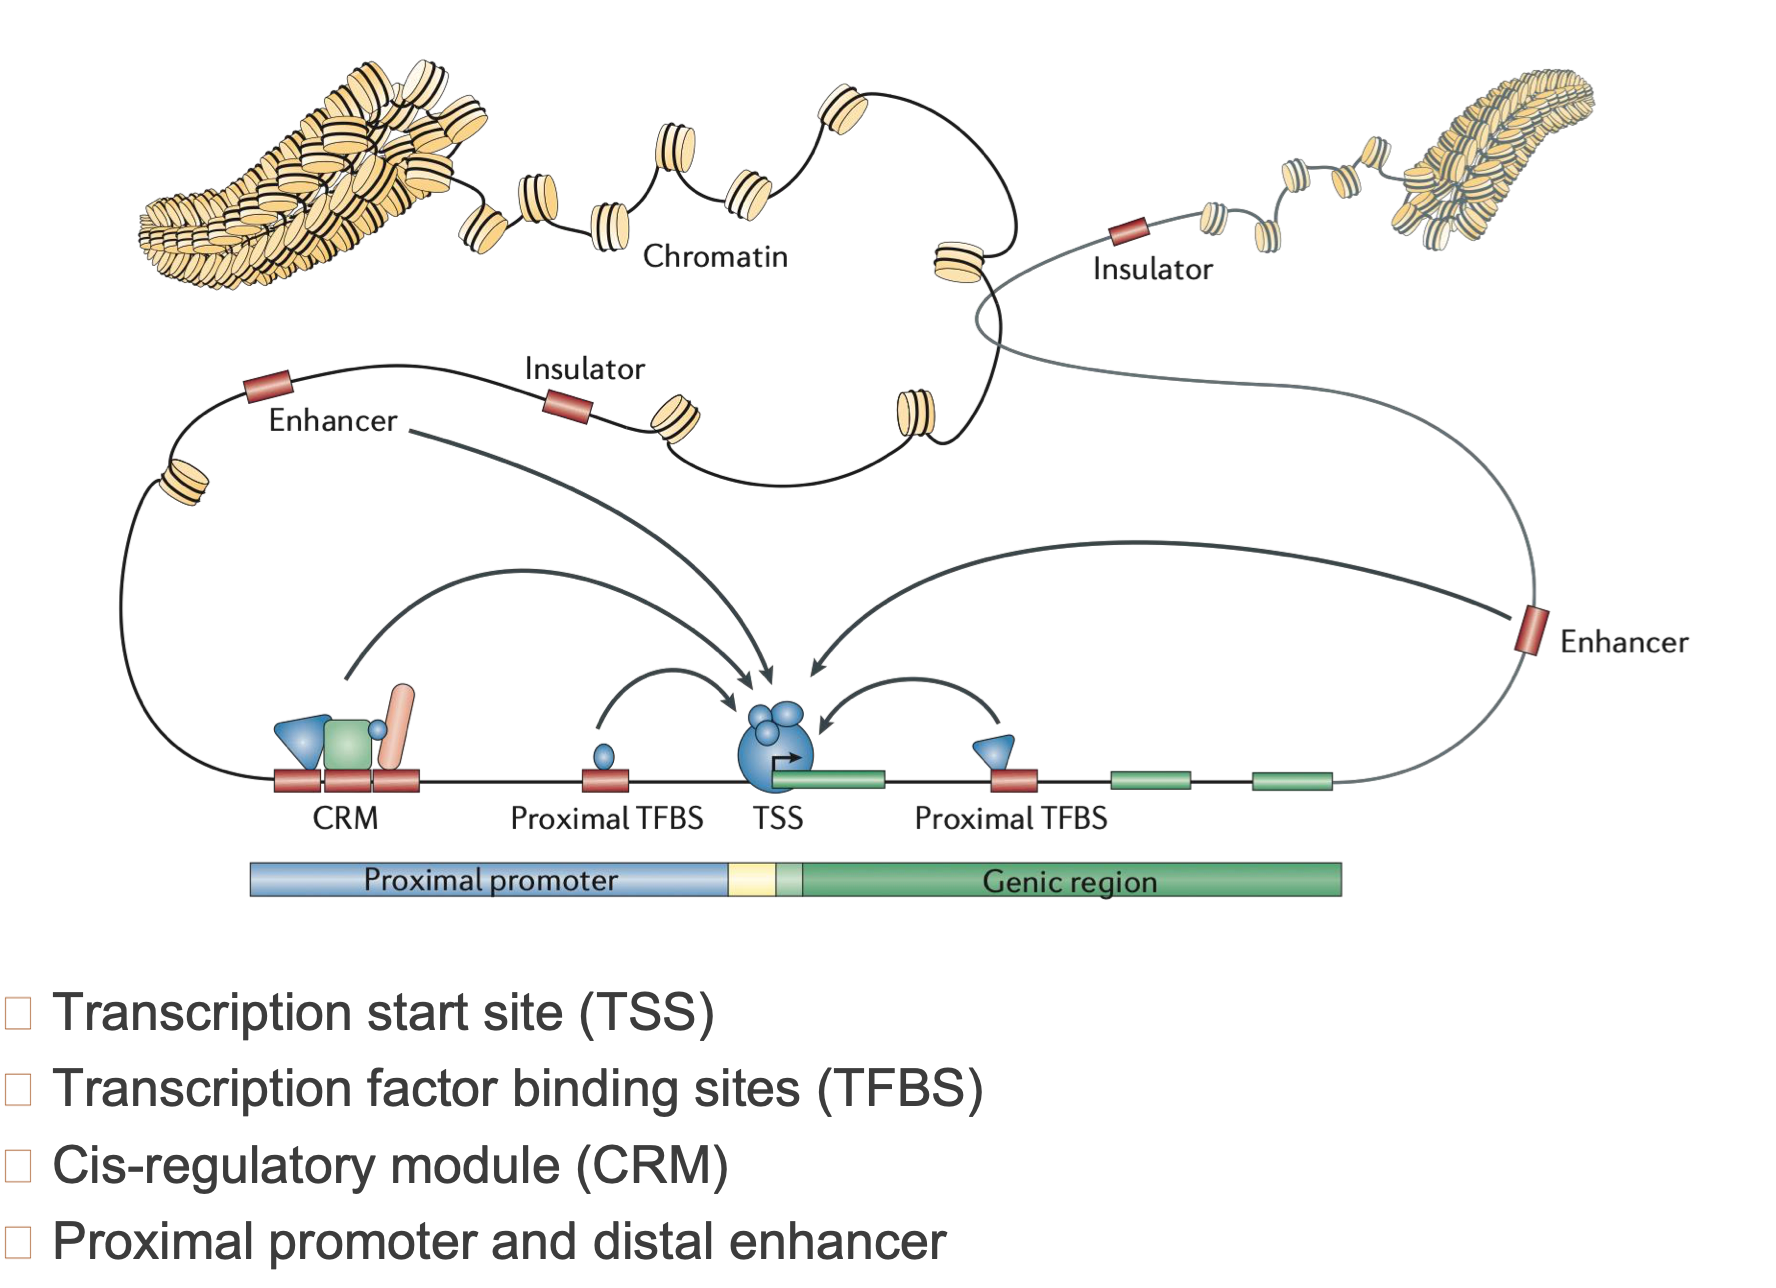
\includegraphics[width=0.6\linewidth]{TFillustration}
		\label{fig:tfillustration}
	\end{figure}
	\item The core promotor regions has about 300 TF, \\
	(general transcription machinery, required for the transcription of most things), \\
	another 1500 TFs for others (proximal enhancer/promotor/silencer, only affect some genes)
	\item comparisons of different whole genome enrichment technologies
	\begin{figure}[h!]
		\centering
		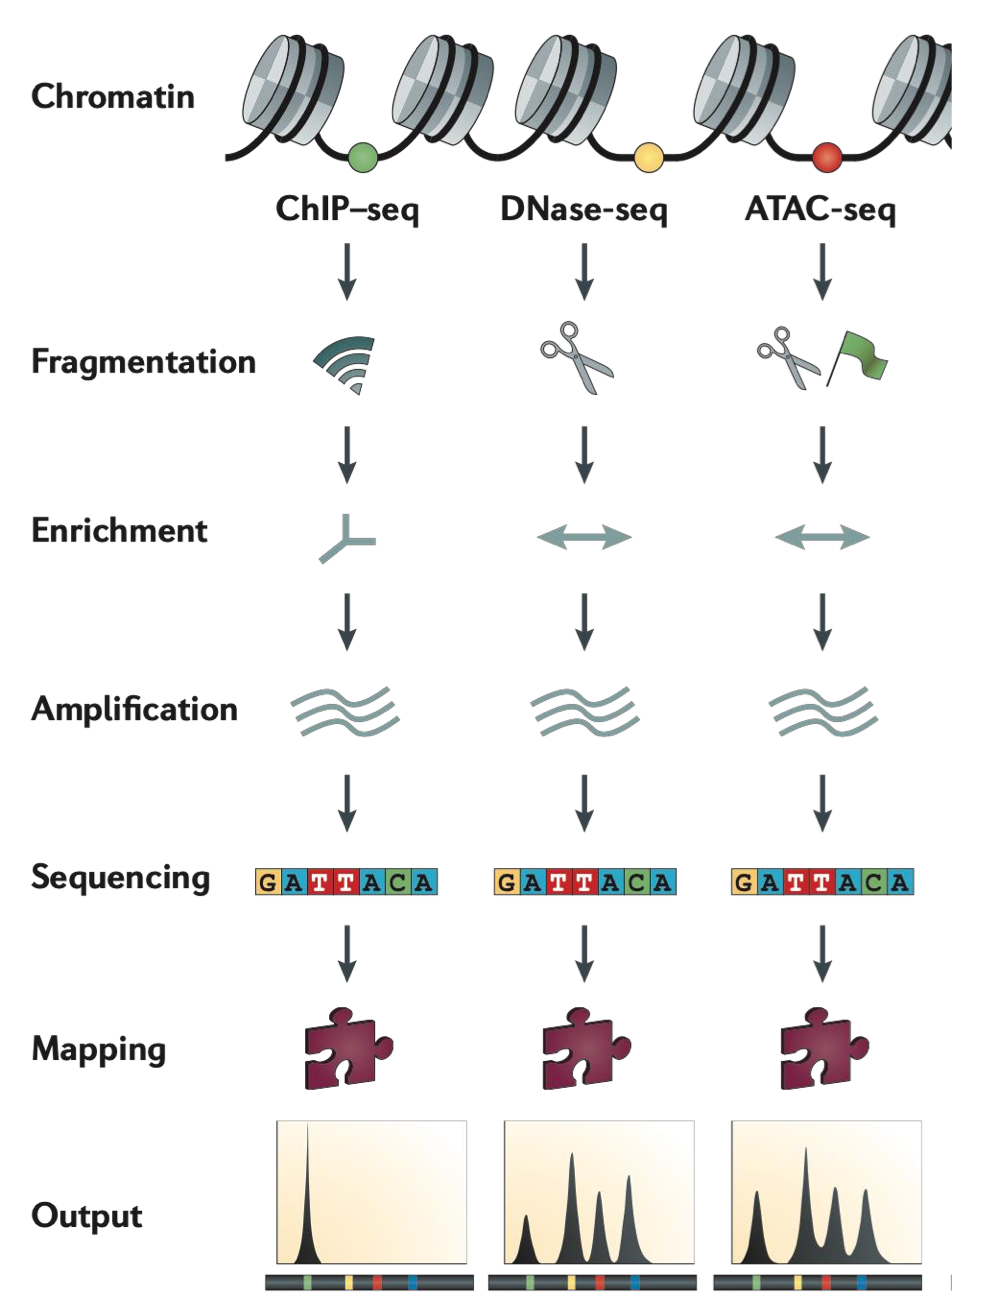
\includegraphics[width=0.4\linewidth]{genomewide_profiling_tech}
		\label{fig:genomewideprofilingtech}
	\end{figure}
	
\end{itemize}
\subsection{Questions related to TF binding}
\begin{itemize}
	\item Where do they bind
	\begin{itemize}
		\item some almost always bind to proximal promotors
		\item others could bind to many regions
	\end{itemize}
	\item How does specific binding work
	\begin{itemize}
		\item exists a consensus motif (most common sequence)
		\item looks like this 
		\begin{figure}[h!]
			\centering
			
\includegraphics[scale=0.2]{concensusmotif}
			\label{fig:concensusmotif}
		\end{figure}
		\item shows which nucleotide is most abundant at each position, represented as \kyw{Position Weight Matrix (PWM)}
		\item \textcolor{red}{Motif}: a \kyw{recurring} sequence with biological importance
			\begin{itemize}
				\item can be constant or have a feww variable elements
				\item often serves as binding site for TFs /proteins
				\item often very short (5-25)
				\item often distant from gene
				\item  often has inexact repeating pattern (challenge for identification)
			\end{itemize}
		\item sometimes also an effect of protein-protein interactions,\\
			ie. protein conformation change upon interactions etc?
		\item to determine binding site, often uses \textcolor{red}{Protein Weight Matrix}, but it is over-simplifying
		\end{itemize}
	\item How to identify where they bind
		\begin{itemize}
			\item genes regulated by the same TF are likely to have the same motif in regulatory region
			\item to find genes regulated by the same TF $\rightarrow$ \cmt{comparative genomics} could be very useful
			\item eg. knock-off of specific TFs $\rightarrow$ lower expression of a set of genes
			\item group of genes that are co-expressed across many set of experiments are also likely to be regulated by same TF
			\item challenges
				\begin{itemize}
					\item we don't know the exact motif seq
					\item we don't know how far it will be
					\item motifs can differ slightly across
					\item how to distinguish it from just ``random'' sequences that happen to repeat?
				\end{itemize}
			\item Multiple sequence alignment (MSA)
			\item motif-finding based on EM algorithm (MEME-suite - Multiple EM for Motif Elucidation)
		\end{itemize}
	\item How is it involved in gene regulation
	\item Is it useful for gene regulatory network?
\end{itemize}
\subsection{ChIP-seq}
\begin{itemize}
	\item technology:\\
	\kyw{ChIP}: chromatin immunoprecipitation\\
	studies protein interaction with DNA\\
	able to map global binding site precisely for any protein of interests
		\begin{enumerate}
			\item chromatin immunoprecipitation + high throughput sequencing
			\item detect genome-wide location of TF and other binding proteins in labs
			\item find all DNA seq bound by TF-X
			\item try to learn the regulatory mechanisms of a TF or DNA-binding protein
		\end{enumerate}
	\item General strategies to call ChIP-seq peaks
		\begin{itemize}
			\item ChIP-seq yields distributions for tags from forward and reverse strands
			\item overlap of the two can be observed
			\item actual binding site of TF should be between the 2 distributions
			\item from the difference between the 2 peaks $\rightarrow$ formulate a single \kyw{peak summit}  
		\end{itemize}
	\item MACS: model-based analysis for ChIP-seq
	\begin{enumerate}
		\item map reads using Bowtie2
		\item get ChIP-seq reads around but may not contain binding site
		\item sequence are from ends of randomly chopped segments $->$ hopefully overlap at binding site
		\item produce 2 adj. set of read peaks located about $ 2\times $ fragment length away
		\item \kyw{shift distance}: dist between read peaks at which will find true peak
		\item automatically subtract control to define a final set of peaks
	\end{enumerate}
	\begin{itemize}
		\item input: \\
		bandwidth : sonication size\\
		mfold: high-confidence fold enrichment
		\item slides $ 2\times $ bandwidth window across genome to find regions with tags $ > mfold$ enriched compared to a random tag
		\item random sample 1000 high quality peaks, separate their Watson Crick tags, and align by midpoint $->$ 2 peaks, shifts = $ d/2 $
		\item tag distribution $ ~ Poisson $
		\item MACS uses a dynamic parameter $ \lambda_{local} $
		\item \cmt{P-val of peaks?}
		\item \cmt{FDR?}
	\end{itemize}
	\item Downstream analysis
	\begin{itemize}
		\item to identify motif for TF using ChIP-seq peaks -- \kyw{MEME}
		\item to find out what the sequence motifs resembles -- \kyw{TomTom}
		\item to find peak regions of known motifs -- \kyw{FIMO}
		\item look up biological pathways or functions of target genes of TF --\kyw{GREAT}
	\end{itemize}
	\item Practical pipeline
	\begin{itemize}
		\item overview: TF-binding $\to$ co-factors $\to$ DNA histone modifications $\to$ DNA DS break
		\item goal: converg NGS reads to singals / peaks tracks $\to$ infer potential TF binding regions\\
		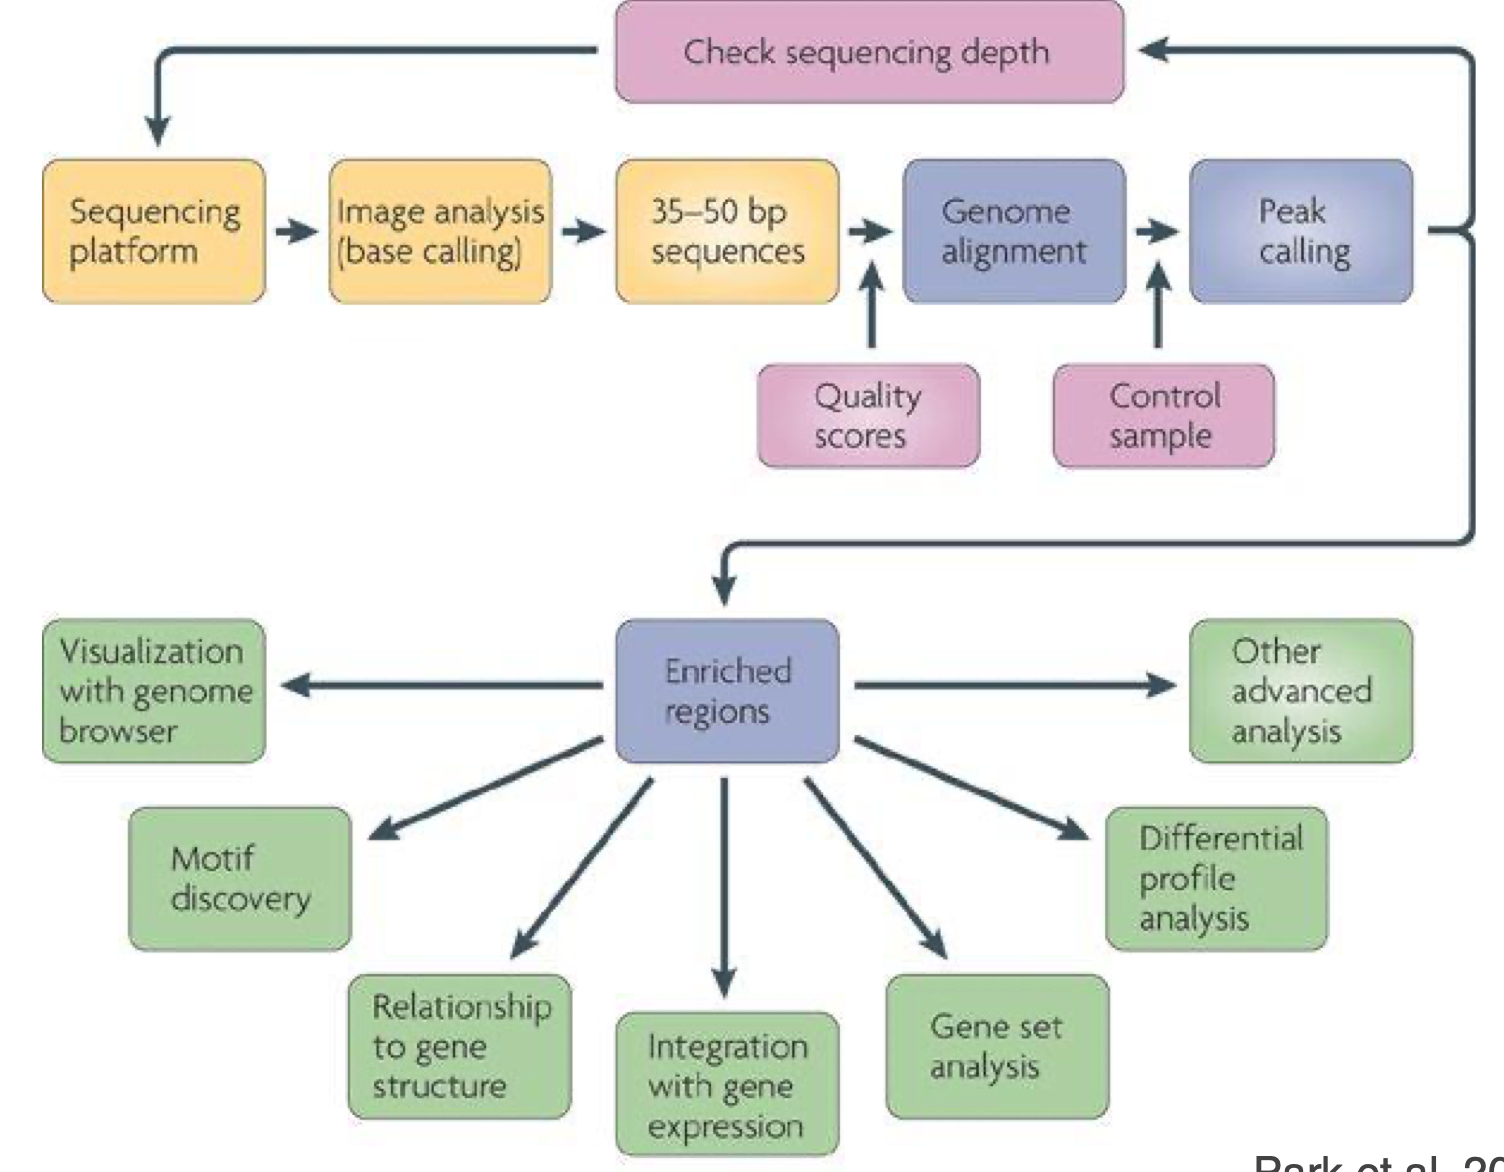
\includegraphics[width=0.7\linewidth]{chipseqpipeline}
		\item fastq $\to$ FASTQC $\to$ bam/alignment \\
		$\to$ wig:\\
		- narrow $\to$ narrow peak caller\\
		----calculate QC matrics\\
		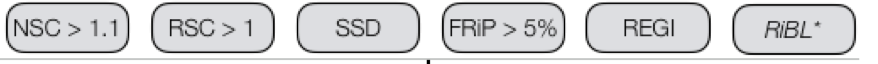
\includegraphics[width=0.7\linewidth]{narrowpeakcaller1}\\
		- broad / mixed $\to$ broad peak caller
		----calculate QC matrics\\
		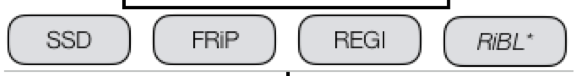
\includegraphics[width=0.45\linewidth]{broadpeakcaller}\\
		\item QC good $\to$ differential enrichment
		\item QC bad $\to$ combine replicates (IDR)
	\end{itemize}
	\item Steps: (eg. ENCODE)
	\begin{enumerate}
		\setcounter{enumi}{-1}
		\item experiment design \\
		- replicates (more replicates $ >> $ greater coverage)\\
		if more TF targets $\to$ multiple hypothesis testing???
		- choice of control
		\begin{itemize}
			\item open-chromatin regions fragmented more easily than closed ones
			\item copy number variation in cancer samples
			\item potential non-specific antibody binding
			\item repetitive regions could cause alignment errors
			\item MOST DO CONTROL AS PART OF THE INPUT
			\item some also do mock IP as control (DNA obtained from IP by a mock antibody such as IgG)
		\end{itemize}
		* \textbf{matched control} is required for downstream analysis
		\item input data \& QC
		\begin{itemize}
			\item fasta format $\to$ FastQC
		\end{itemize}
		\item Aignment and filtering
		\begin{itemize}
			\item alignment tools: bowtie, bwa$\to$output bam
			\item QC = \% mapped
			\item filtering tools: samtools, picard
			\item QC = non-redundant fraction
		\end{itemize}
		\item Peak calling
		\begin{itemize}
			\item narrow peak
			\item broad peak
			\item QC: fraction of reads in peak (FRiP)
			\begin{itemize}
				\item FRiP values correlate positively and linearly with the number of called regions
			\end{itemize}
			\item QC: strand cross-correlation
			\begin{itemize}
				\item shift vectors with each other and calculate correlations
				\item plot shift size w correlation
			\end{itemize}
			\item Irreproduncibility discovery rate (IDR)
			\begin{itemize}
				\item avoid of choices of initial peak caller cutoffs
				\item modelling peaks pairs from replicates as belonging to two groups: reproducible group and irreproducible group
			\end{itemize}
			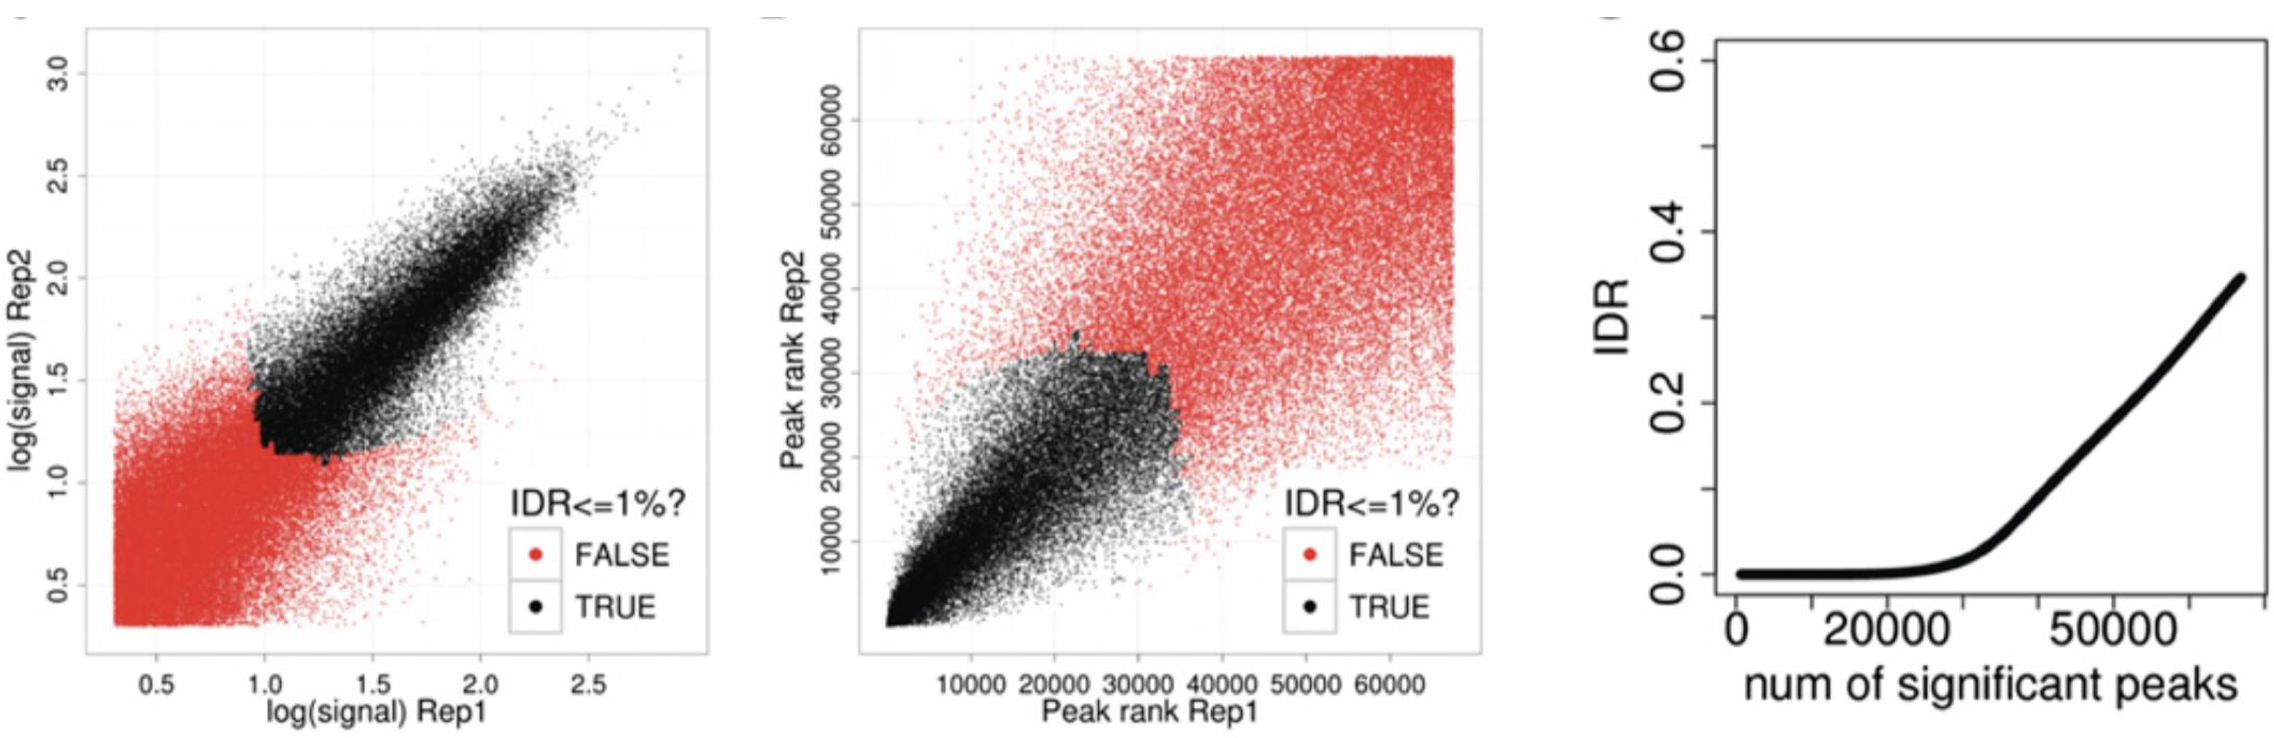
\includegraphics[width=\linewidth]{IDR}
			\item visualization
			\begin{itemize}
				\item UCSC genome browser etc
				\item IGV genome browser
			\end{itemize}
		\end{itemize}
	\end{enumerate}
\end{itemize}

\newpage
\section{cis-regulatory motif}
\subsection{Background of transcription factor binding motif analysis}
\begin{itemize}
	\item basic for TF binding, where they bind
	\item Position weight matrix (PWM)
	\item \textit{De novo} motif binding
	\begin{itemize}
		\item comparative genomic approach $\to$ find motifs within same species
	\end{itemize}
\end{itemize}

\subsection{Finding regulatory motifs}
\begin{itemize}
	\item goal: given a set of genes that are probably regulated by the same TF, find the TF-binding motif in common
	\item challenges: \begin{itemize}
		\item we don't know the sequence of motifs
		\item it could be located near or far
		\item motifs could differ slightly from one to another
	\end{itemize}
	\item assumptions: \begin{itemize}
		\item functional part of genome evolve more slowly than non-functional part $\to$ greater selection pressure
		\item sequence alignment $\to$ identify conserved region
		\item look for functional features in conserved regions
		\item comparative genomics rely on being able to detect similar regions across genomes
	\end{itemize}
\end{itemize}

\subsection{Motif finding based on EM}
\begin{itemize}
	\item E step: fill in the expected values of the misssing variable
	\item M step: regular MLE using the value computed in the E step and values of the other variables
	\item guarantee convergence to local optima
	\item eg. MEME uses EM to iteratively refine \textcolor{blue}{PWM} and identifying sites for each PWM\
	\begin{enumerate}
		\item estimate motif model (PWM)
			\begin{itemize}
				\item start witha k-mer seed (random, or specific
				\item build PWM by incorporating some background frequencies
				\item eg. build a matrix with 4 rows and $k$ cols where each col corresponds to an index 
			\end{itemize}
		\item identify examples of the model
			\begin{itemize}
				\item for every k-mer in input, identify its prob. given the PWM
				\item eg. score all k-mers using a sliding window with the current matrix
			\end{itemize}
		\item  re-estimate the motif model
			\begin{itemize}
				\item calculate new PWM based on the weighted frequencies of all k-mers in input sequence
				\item eg. more likely k-mer from step 2 count more towards new PWM freq. the new PWM is estimated based on the weighted contribution of all k-mers
			\end{itemize}
		\item  iteratively refine the PWMs and identifying sites until convergence
	\end{enumerate}
	\item a bit more formally
	\item input:
		\begin{itemize}
			\item a set of sequences $s_1\cdots s_N$
			\item partition $s$ into k-mers for a fixed k
			\item set of letters, usually assumed to be $\{A,T,C,G\}$
		\end{itemize}
	\item params of the mixture model: $\lambda_1\theta_1 +\lambda_2\theta_2$
		 \begin{itemize}
			 \item  TF motif model $\theta_1$
			 \item background model $\theta_2$
			 \item model probabilities: $\lambda_1, \lambda_2$
		\end{itemize}
\end{itemize}

\subsection{Transform a PWM into log likelihoods}
\begin{itemize}
	\item  to score a single site $s$ for motif $M$, we use  $\Pr(s|M)$, which is the PWM  
	\item easy to calculate the probability for any seq. and motif
	\item to take bg freq into acct, divide by bg freq, and log to make it additive\[\log_2\dfrac{\Pr(s|M)}{\Pr(s|M_{bg})}\]
	\item score = sum of the corresponding entries in the PWM for each position and each letter
\end{itemize}

\subsection{Comparative genomics - PhyloCon}
\begin{itemize}
	\item Align two profiles
	\item each col $\to$ base count $ (n_A, n_C, n_G, n_T) \to (f_A, f_C,f_G,f_T)$
	\item log-likelihood ratio = $ \sum_{\text{base }b} n_{bj}\ln (f_{bi}/p_b)  $ measures likelihood of observed data from col $J$ being generated by dist. estimated by column $i$\\
	* not all regulatory elements are conserved\\
\end{itemize}

\newpage
\section{Haplotype inference}
\subsection{Phase}
\begin{figure}[h!]
	\centering
	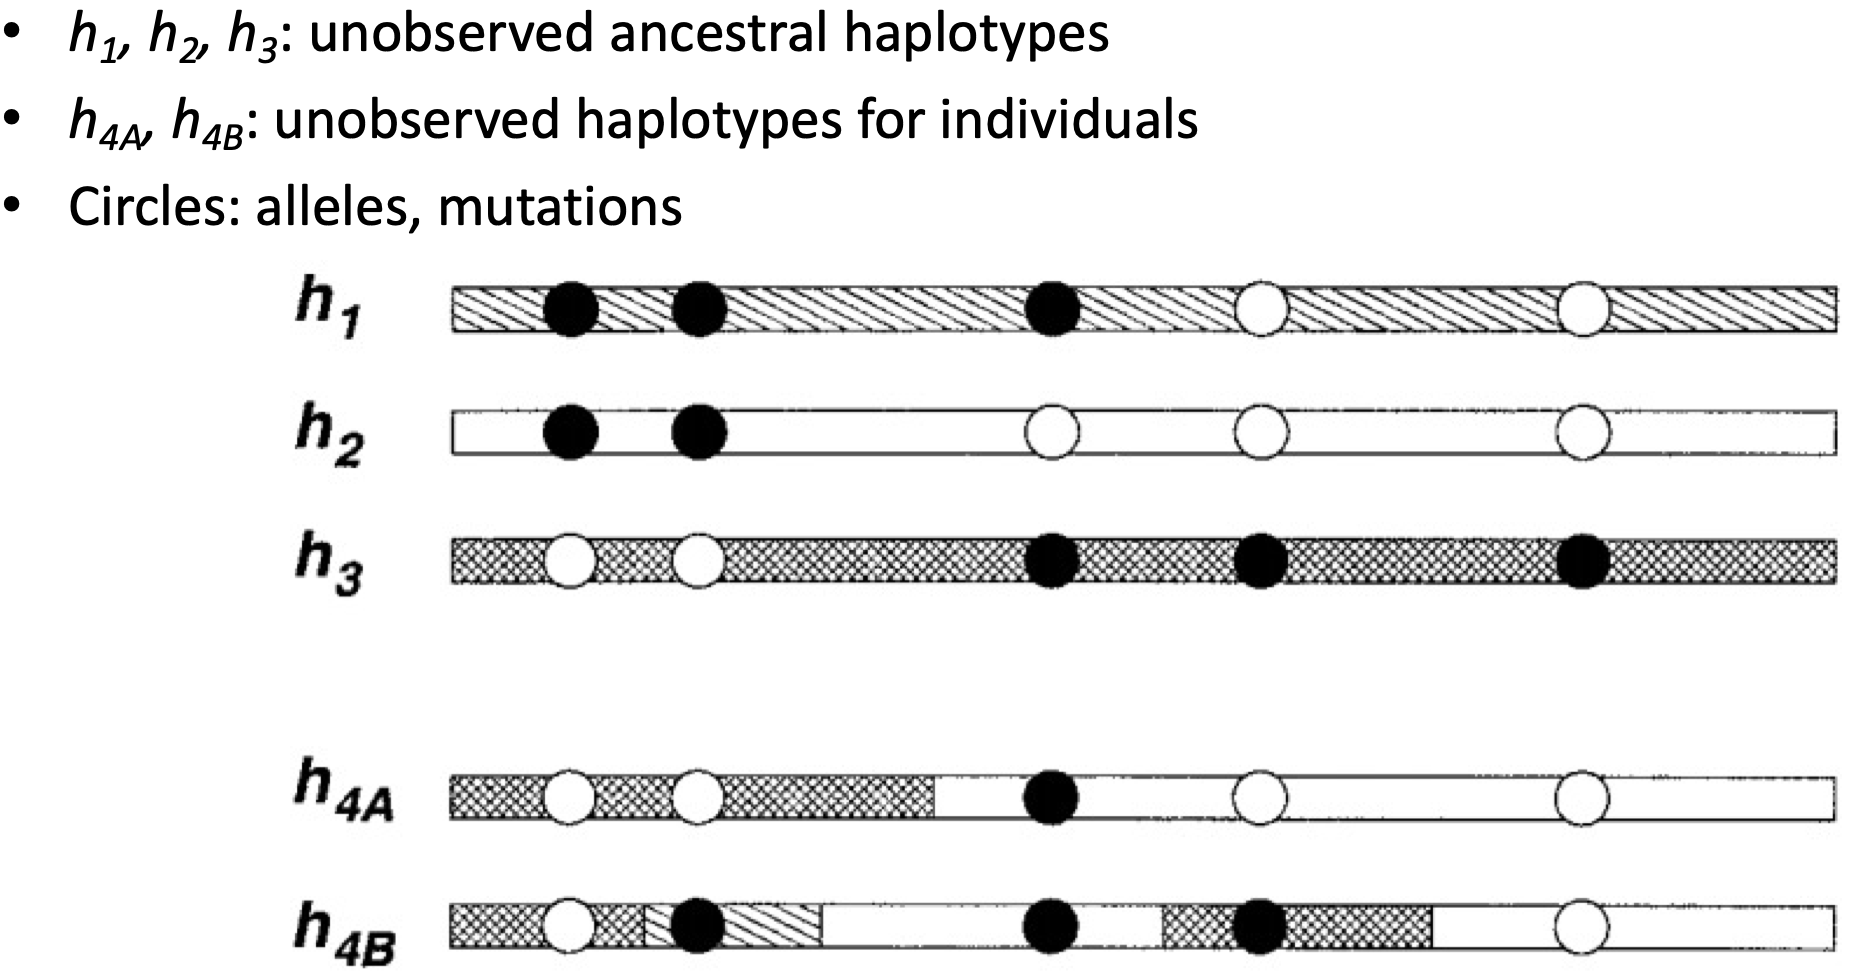
\includegraphics[width=0.7\linewidth]{phase}
	\label{fig:phase}
\end{figure}

\begin{figure}[h!]
	\centering
	\includegraphics[width=0.7\linewidth]{"haplotype structure"}
	\label{fig:haplotype-structure}
\end{figure}
\begin{itemize}
	\item Genotype inputation
	\begin{itemize}
		\item Given: SNP array genotype data
		\item some has missing data / untyped SNPs
		\item much cheaper
		\item use HMM
		\item more data, more acurate for inputation
	\end{itemize}
	\item Beagle / SHAPE-IT are most commonly used software
\end{itemize}
\subsection{Linkage disequilibrium (LD)}
\begin{itemize}
	\item reflect rs between alleles at diff loci
	\begin{itemize}
		\item linkage equilibrium: no linkage, not coupled
		\item disequilibrium $ \rightarrow $ linkage
	\end{itemize}
	\item \kyw{LD:} allelic association meansure
	\item calculating LD:
	\begin{itemize}
		\item assume independence, calculate expected frequency
		\item $ D_{AB} = P_{AB} - P_A P_B $
	\end{itemize}
	\item calculate for all loci (SNPs)
	\item spot-light figures\begin{figure}[h!]
		\centering
		\includegraphics[scale = 0.2]{"chromosome spotlight"}
		\label{fig:chromosome-spotlight}
	\end{figure}
	\item neighboring loci shows more linkage\\
	there could be LP blocks on the chromosome, where there's stronger linkage within block and weaker across block\\
	each block is like a voting district / \kyw{Marker regions}
	\item They are \cmt{Tag SNPs}
	\item pretty standard practice
	\item dense genotyping more expensive 
	\begin{itemize}
		\item get the LP
		\item use inference on sparser genotyping 
		\item multi-phase procedure
	\end{itemize}
\end{itemize}

\newpage
\section{Population structure}
\subsection{Background}
\begin{itemize}
	\item def: set of individuals with distinct genetic variations
	\item eg. ancestral history, lactose intolerance
	\item Hardy-Weinburg equilibrium
	\begin{itemize}
		\item Under random mating, both allele and genotype frequency remain const
		\item Current gen:
		\begin{itemize}
			\item $ D + H + R = 1 $
			\item $ p = \frac{2D + H}{2} $
			\item $ q = \frac{2R + H}{2} $
		\end{itemize}
		\item Next gen:
		\begin{itemize}
			\item $ D' = p^2 $
			\item $ H' = 2pq $
			\item $ R' = q^2 $
			\item $ p' = \frac{2p^2 + 2pq}{2} = p^2 + pq = p $
			\item $ q' = \frac{2p^2 + 2pq}{2} = q^2 + pq = q$
		\end{itemize}
		\item given population data, can test if it holds (often chi-square test)
		\begin{itemize}
			\item testing is recommended
			\item if fail, means something is going on
			\item or genotyping error
			\item want HWE to hold for control group
		\end{itemize}
		\begin{enumerate}
			\item compute allele freq from observed data
			\item compute expected genotype freq
			\item compute test statistic (deg of freedom 1)
		\end{enumerate}
		\item Due to \kyw{Genetic drift}, even when assumptions of HWE hold, HWE may not hold
	\end{itemize}
	\item genetic drift
	\begin{itemize}
		\item change in allele freq due to random sampling
		\item all mutations eventually drift to 0 or 1 eventually
		\item is neutral
	\end{itemize}
	\item Wright's $ F_{ST} $ (Wright-Fisher model)\\
	\[ {{2N}\choose{k}} p^k q^{2N-k} \]
	\item Ways how populations evolve
	\begin{itemize}
		\item population divergence\\
		separated into subpopulations with independent selection and drift
		\item admixture\\
		mixing of population
	\end{itemize}
\end{itemize}
\subsection{Infering pop structure from genotype data (nowadays mostly just PCA)}
\begin{itemize}
	\item Mixture model 
	\begin{itemize}
		\item cluster individual into K populations
		\item \cmt{does not model admixture}
		\item cluster individual into populations
		\item probability model for mixture of $ C $ Gaussians
		\[ p(x) = \sum_{i=1}^k p(x|c=i)\cdot p(c=i)\]
		\item $ c $: labels, $ p(c) $ label freq, multinuilli
		\item $ x $: genotype / alleles, $$ p(x|c) = \Pi_{i=1}^j p(x_i|c)$$ , assume independence
		\item can then learn the model with EM
		\item Inference: $p(c|x)$ to infer cluster label
	\end{itemize}
	\item Admixture model
	\begin{itemize}
		\item modern species are mixture of ancestral populations
		\item genome consists of contributions from multiple ancestral populations, eg. Asian, African, Caucassians
		\item want to model it as a mosaic of variant
		\item Assumptiosn
		\begin{itemize}
			\item no linkage disequilibrium
			\item SNPs are iid
		\end{itemize}
		\begin{figure}[h!]
			\centering
			\includegraphics[scale = 0.2]{"admixture.jpg"}
		\end{figure}
		\item for each individual $i: 1\rightarrow n $:
		\begin{itemize}
			\item sample $ \theta_i $ from Dirichlet$ (\alpha) $
			\item for each loci $j: 1 \rightarrow L$
			\begin{itemize}
				\item sample $ Z_{j,i} $ from multinomial $ \theta_n $
				\item sample $ X_{j,i} $ from $ \beta_{k_j} $ for $ k $ chosen by $ k= Z_{j,i} $
			\end{itemize}
		\end{itemize}
	\item still have to go back to $ \beta $
	\item instead of sampling $ p_c $ of population it gets $ p_c $ for each individual
	\end{itemize}
	\item Evaluations
	\begin{itemize}
		\item probabilistic model
		\item is generative process
		\item explanatory, descriptive, and interpretable
		\item computation can be very expensive
	\end{itemize}
	\item PCA
	\begin{itemize}
		\item fast, although not too much information
		\item input: $ N\times L $ for $ N $ individuals and $ L $ loci
		\item good: easy visualization
		\item bad: doesn't give intuition about what is going on, no allele frequency info
	\end{itemize}
\end{itemize}
\newpage
\section{Linkage Analysis, GWAS(Genome Wide Association Study)}
\subsection{Background}
\begin{itemize}
	\item Genome polymorphisms
	\begin{itemize}
		\item human genealogy \imp SNPs \imp haplotypes
		\item useful markers for studying disease association
		\item finding genetic markers that are likely to be linked with the disease locus, instead of finding the disease locus itself (cuz it's hard)
		\item making use of linkage (dis)equilibrium, find those loci with $ r < 0.05 $
	\end{itemize}
	\item linkage analysis
	\begin{itemize}
		\item \cmt{family data}
		\item more likely to have linkage data
		\item Effective for rare diseases
		\item Low resolution on the genomes (only a few recombinations)
		\item \textbf{Parametric linkage analysis:}
		\begin{itemize}
			\item need to specify disease model
			\item Highly effective for Mendelian disease caused by a single locus
			\item usually large pedigree
			\item Founder probabilities (founders: parents not in population)
			\begin{itemize}
				\item thus need to assign distributions to their genotypes
				\item often done with Hardy-Weinburg
				\item genotype of the founder couple assumed independence
			\end{itemize}
			\item children get their genes according to \textbf{Mendel's law}
		\end{itemize}
			\item from genotype \imp phenotype
			\begin{itemize}
				\item complete vs incomplete penetrance
				\begin{align*}
					\Pr{[complete | DD]} &= 1\\
					\Pr{[incomplete | DD]} &< 1
				\end{align*}
			\item 
			\end{itemize}
	\end{itemize}
\end{itemize}

\subsection{GWAS}
\subsection{single SNP association analysis}
\begin{itemize}
	\item \cmt{unrelated individuals}
	\item Easier to find a large number of affected individuals
	\item Effective for common diseases
	\item Relatively high resolution for pinpointing the locus linked to the phenotype
\end{itemize}
\begin{figure}[h!]
	\centering
	\includegraphics[width=0.5\linewidth]{"manhanttan plot"}
	\label{fig:manhanttan-plot}
\end{figure}
\subsection{multimarker association test}
\subsection{using reference datasets for genotype imputation}
\begin{itemize}
	\item reference data: dense SNP data - from dataset eg 1000 genome project
	\item new data = sparser SNP
	\item \kyw{leverage LD} - data after imputation w ref data\begin{figure}[h!]
		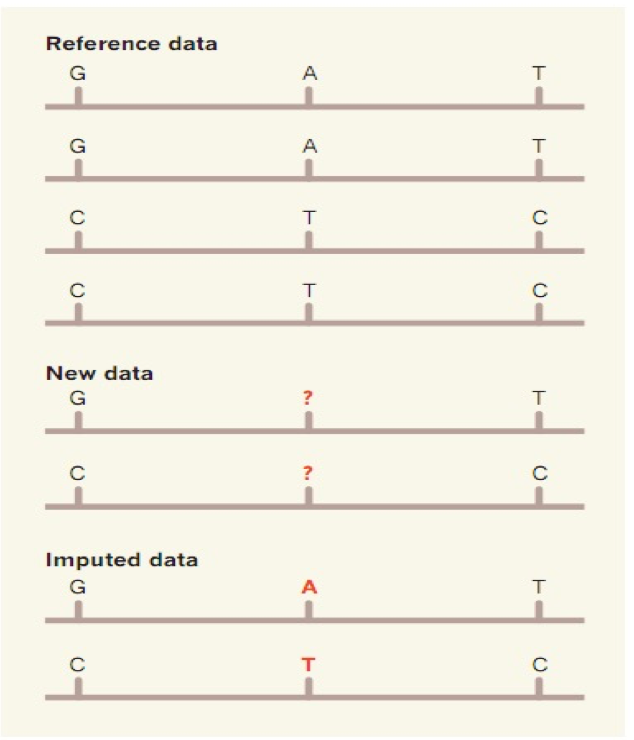
\includegraphics[width=0.3\linewidth]{imputation_data}
		\label{fig:imputationdata}
	\end{figure}\\
	\item imputation based method - everyone is doing it rn \begin{figure}[h!]
		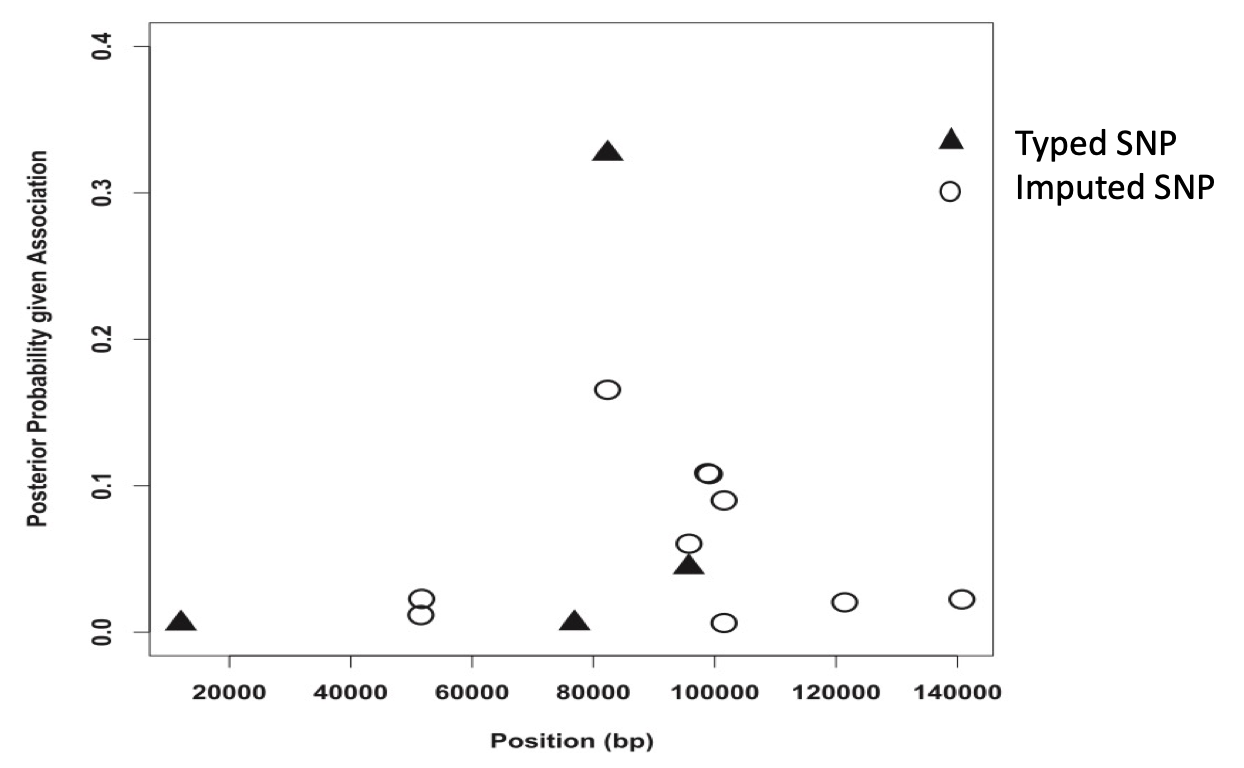
\includegraphics[width=0.5\linewidth]{imputation}
		\label{fig:imputation}
	\end{figure}
	\item association to rare variants (GWAS only mostly apply to common variants)\\
	at least a lot more confident when allele is common\\
	ppl often combine multiple rare alleles along a gene and compare gene
	\item underlying: common allele - common disease / common hypothesis -- assumption \\
	usually 5\% considered ``common'', 0.5\% - 5\% considered ``low frequency variant'', else ``rare variant''
	\item still quite a lot of variant to analyze
	\item feasibility of detecting disease loci\begin{figure}[h!]
		\centering
		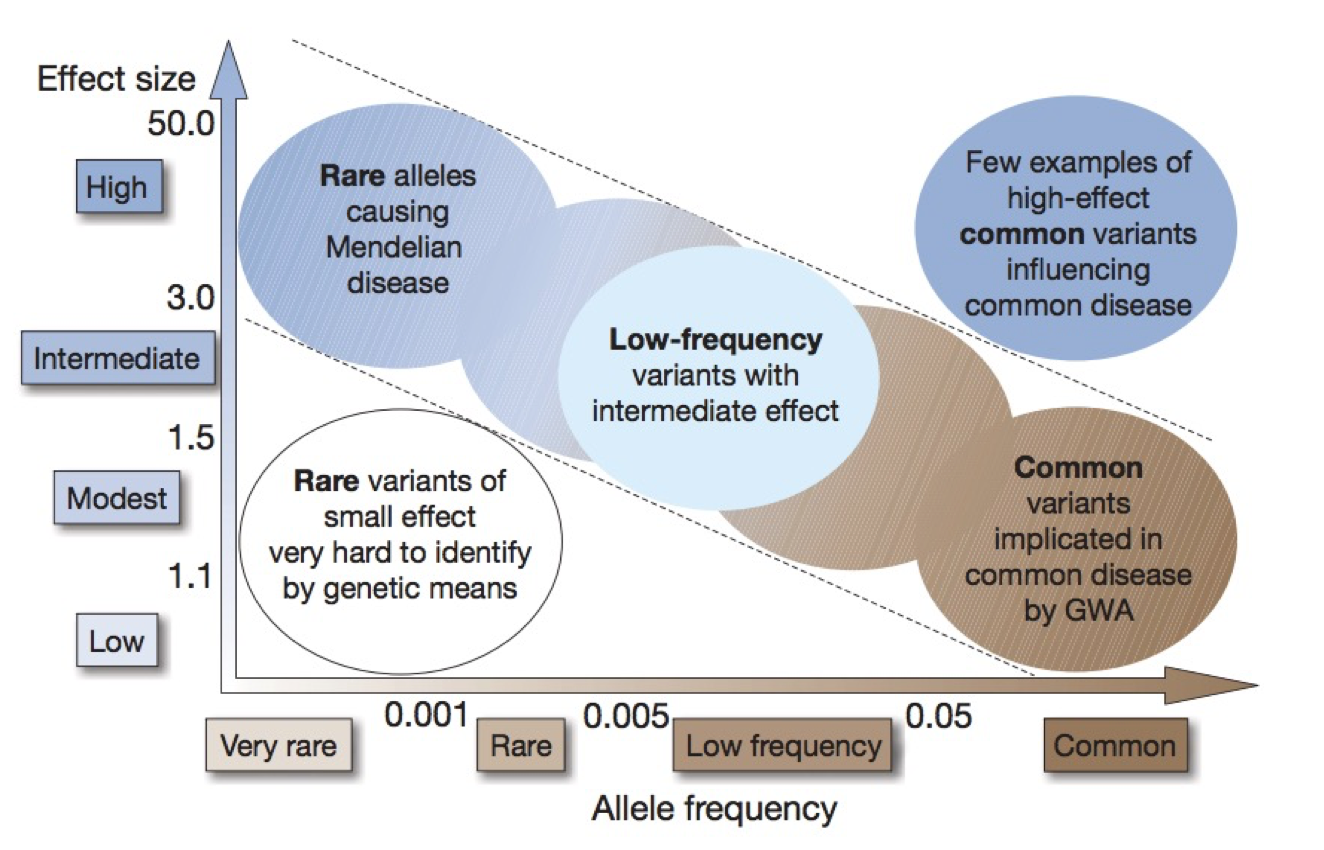
\includegraphics[width=0.5\linewidth]{feasibility.png}
		\caption{}
		\label{fig:feasibilitygwasloci}
	\end{figure}
\end{itemize}
\subsection{Epistasis}
\begin{itemize}
	\item effect of one locus masks another loci\begin{figure}[h!]
		\centering
		\begin{subfigure}[b]{0.6\linewidth}
		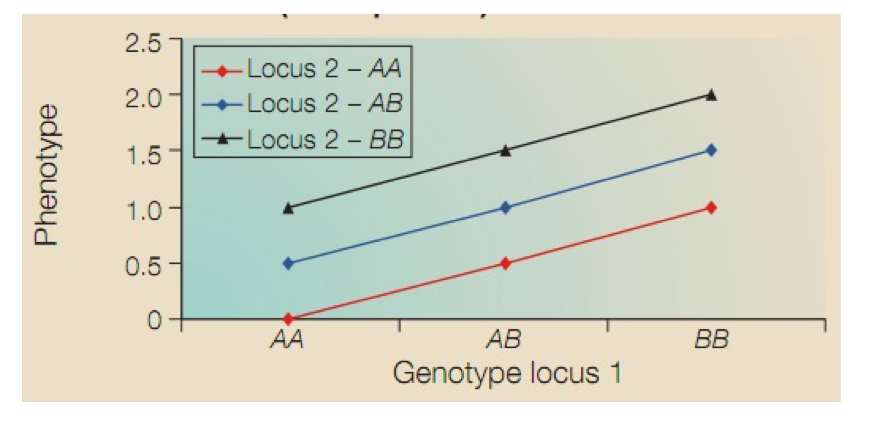
\includegraphics[width=0.6\linewidth]{noepistasis}
		\centering
		\caption{no epistasis}
		\label{fig:noepistasis}
		\end{subfigure}
		\begin{subfigure}[b]{\linewidth}
		\centering
		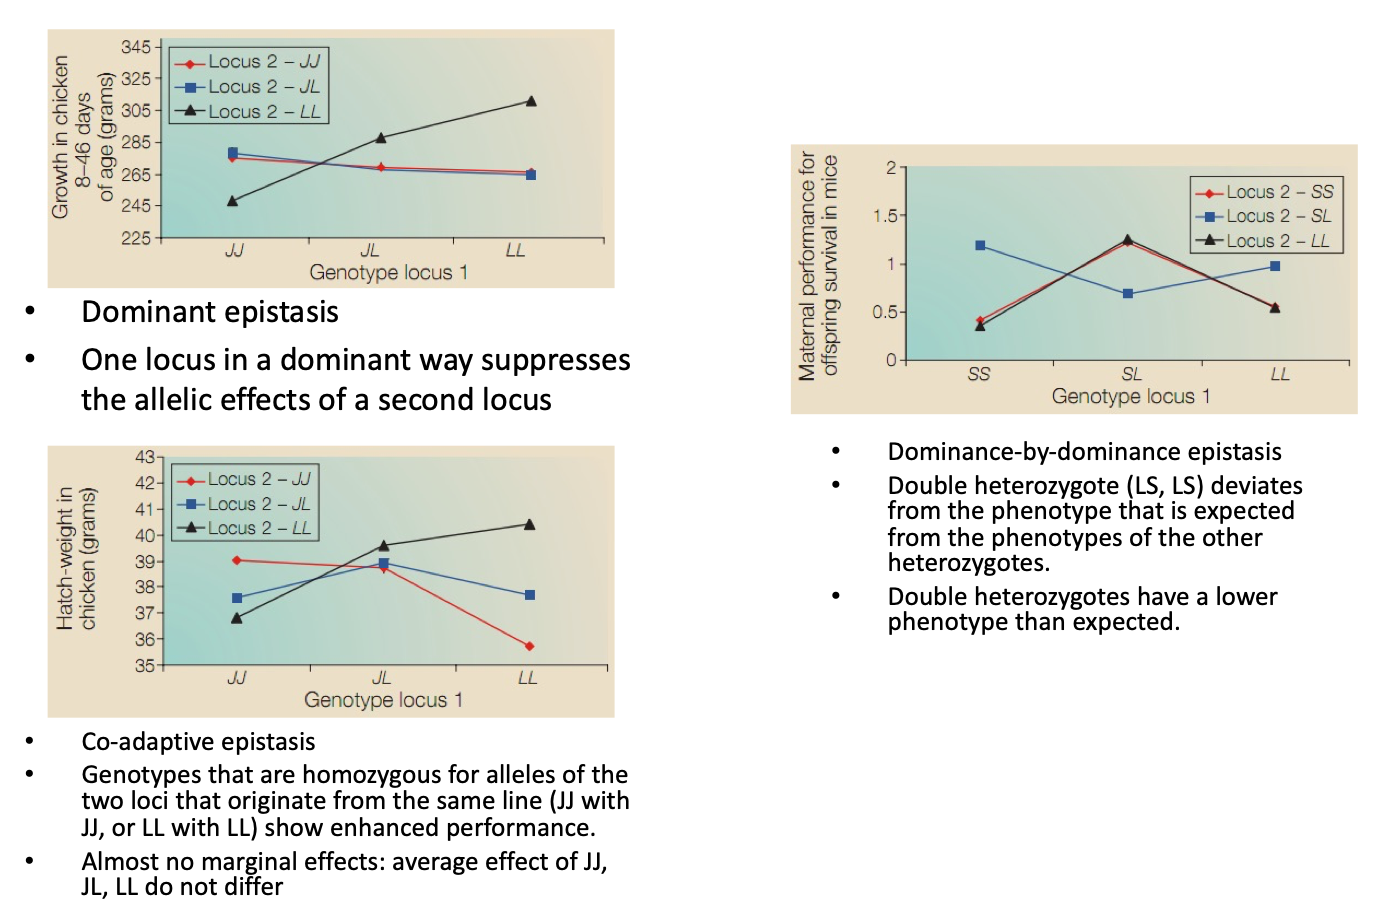
\includegraphics[width=0.7\linewidth]{epistasis}
		\caption{epistasis}
		\label{fig:epistasis}
	\end{subfigure}
	\end{figure}
	\item hard to detect - only if the interacting SNPs are considered jointly
	\item also suffer from multiple testing problem
\end{itemize}

\subsection{Population struture and association analysis}
\begin{itemize}
	\item pop structure can cause false positives
	\begin{itemize}
		\item samples in case are often more related 
		\item Any SNPs more prevalent in the case population will be found significantly with the case 
		\item may capture both disease and population related SNPs
		\item ideally have equal proportion of population in case and control
	\end{itemize}
	\item computationally solve the problem
	\begin{itemize}
		\item poputation based method
		\item Eigenstrat: PCA based method
		\begin{enumerate}
			\item inferring ancestry - PCA applied\\
			infer continuous axis
			\item removing ancestry effects\\
			genotype at candidate SNP adjust by amounts attributable to ancestry along each axis\\
			scaling factor: regression on genotype - ancestral info\\
			\cmt{missing eqns from notes}
			\item association tests
		\end{enumerate}
		\item linear mixed model
	\end{itemize}
\end{itemize}
\newpage
\section{eQTL (expression quantitative trait locus)}
\subsection{limitation of likage analysis and GWAS}
\begin{itemize}
	\item we often know the genetic loci
	\item but don't know the molecular mechanism
	\begin{figure}[h!]
		\centering
		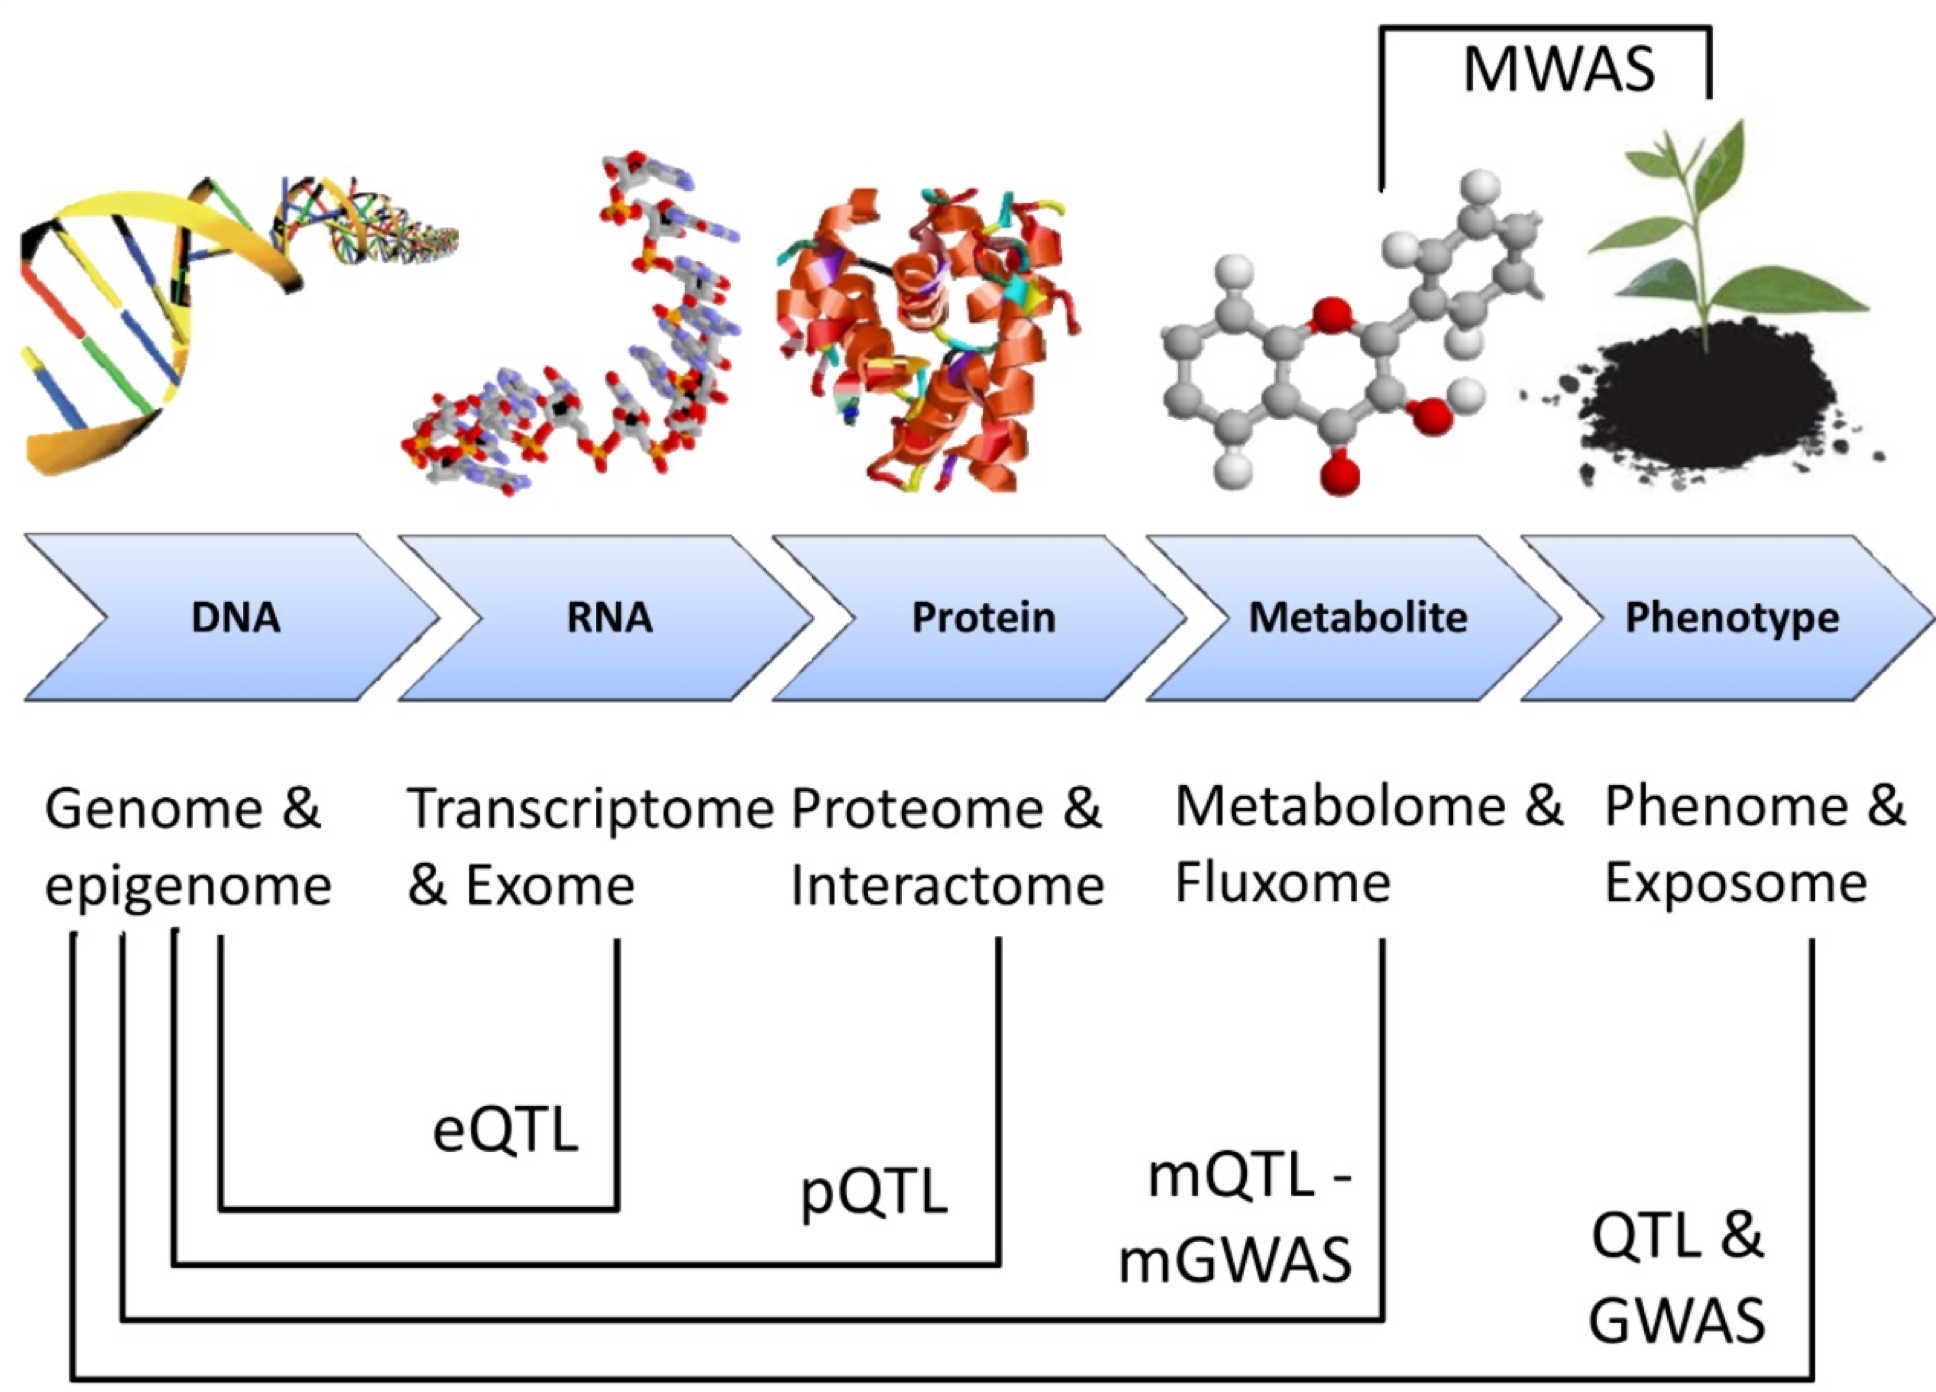
\includegraphics[width=0.4\linewidth]{eqtloverview}
		\label{fig:eqtloverview}
	\end{figure}
	\item find connection between DNA and mRNA
	\item eQTL mapping \begin{figure}[h!]
		\centering
		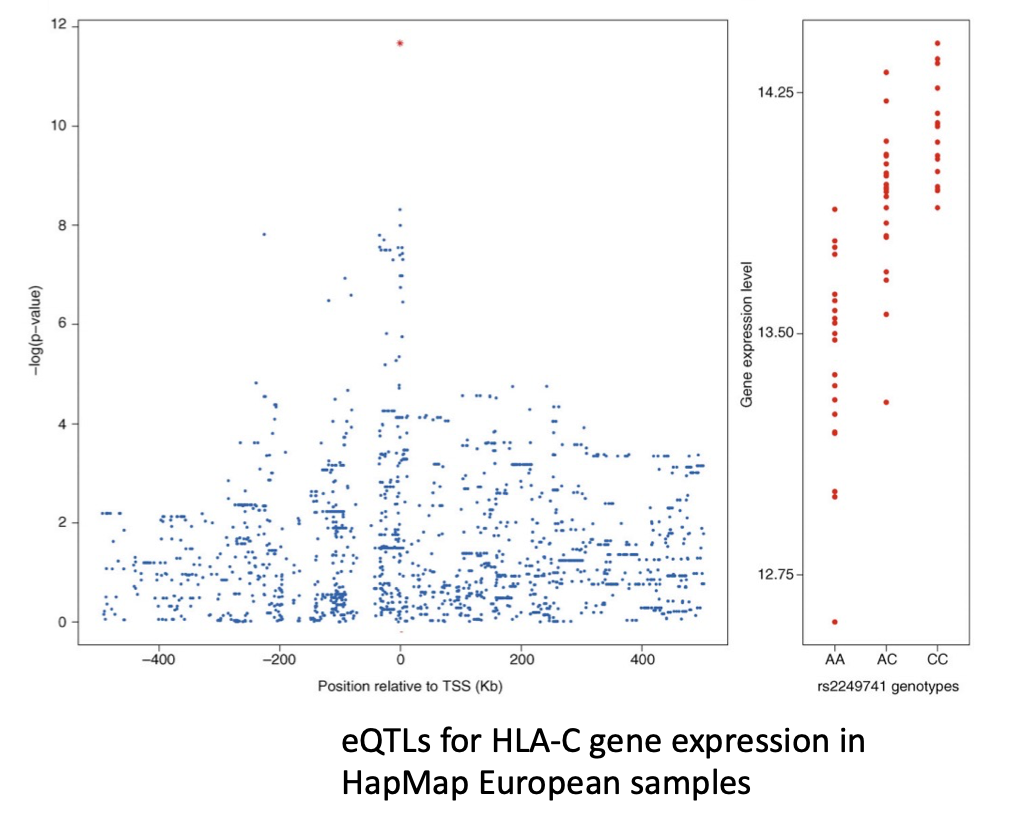
\includegraphics[width=0.5\linewidth]{eqtlmappingeg}
		\label{fig:eqtlmappingeg}
	\end{figure}
	\item genometype tissue expression (GTEx) project
	\begin{itemize}
		\item goal: characterize molecular function of human genome
		\item postmortem samples from normal, non-disease tissues -> reference data
	\end{itemize}
	\item popular tool to study genetic basis of expression for 
	\begin{itemize}
		\item diff tissue types
		\item diff diseases
	\end{itemize}
\end{itemize}
\subsection{terminologies}
\begin{itemize}
	\item \kyw{eGene} genes whose expression is affected by eQTLs
	\item \kyw{cis eQTL} in the genome, the eQTL is located \cmt{near} the eGene\\
	– E.g.,mutations in the promoter region of a gene influence the expression level of the gene\\
	-- but enhancers can be far away, may look like trans
	\item \kyw{trans eQTL} eQTL is located \cmt{far away} (or on a different chromosome) \\
	– E.g.,mutationsinthetranscriptionfactorgene\\
	* cis regulatory can have downstream effect -> trans \begin{figure}[h!]
		\centering
		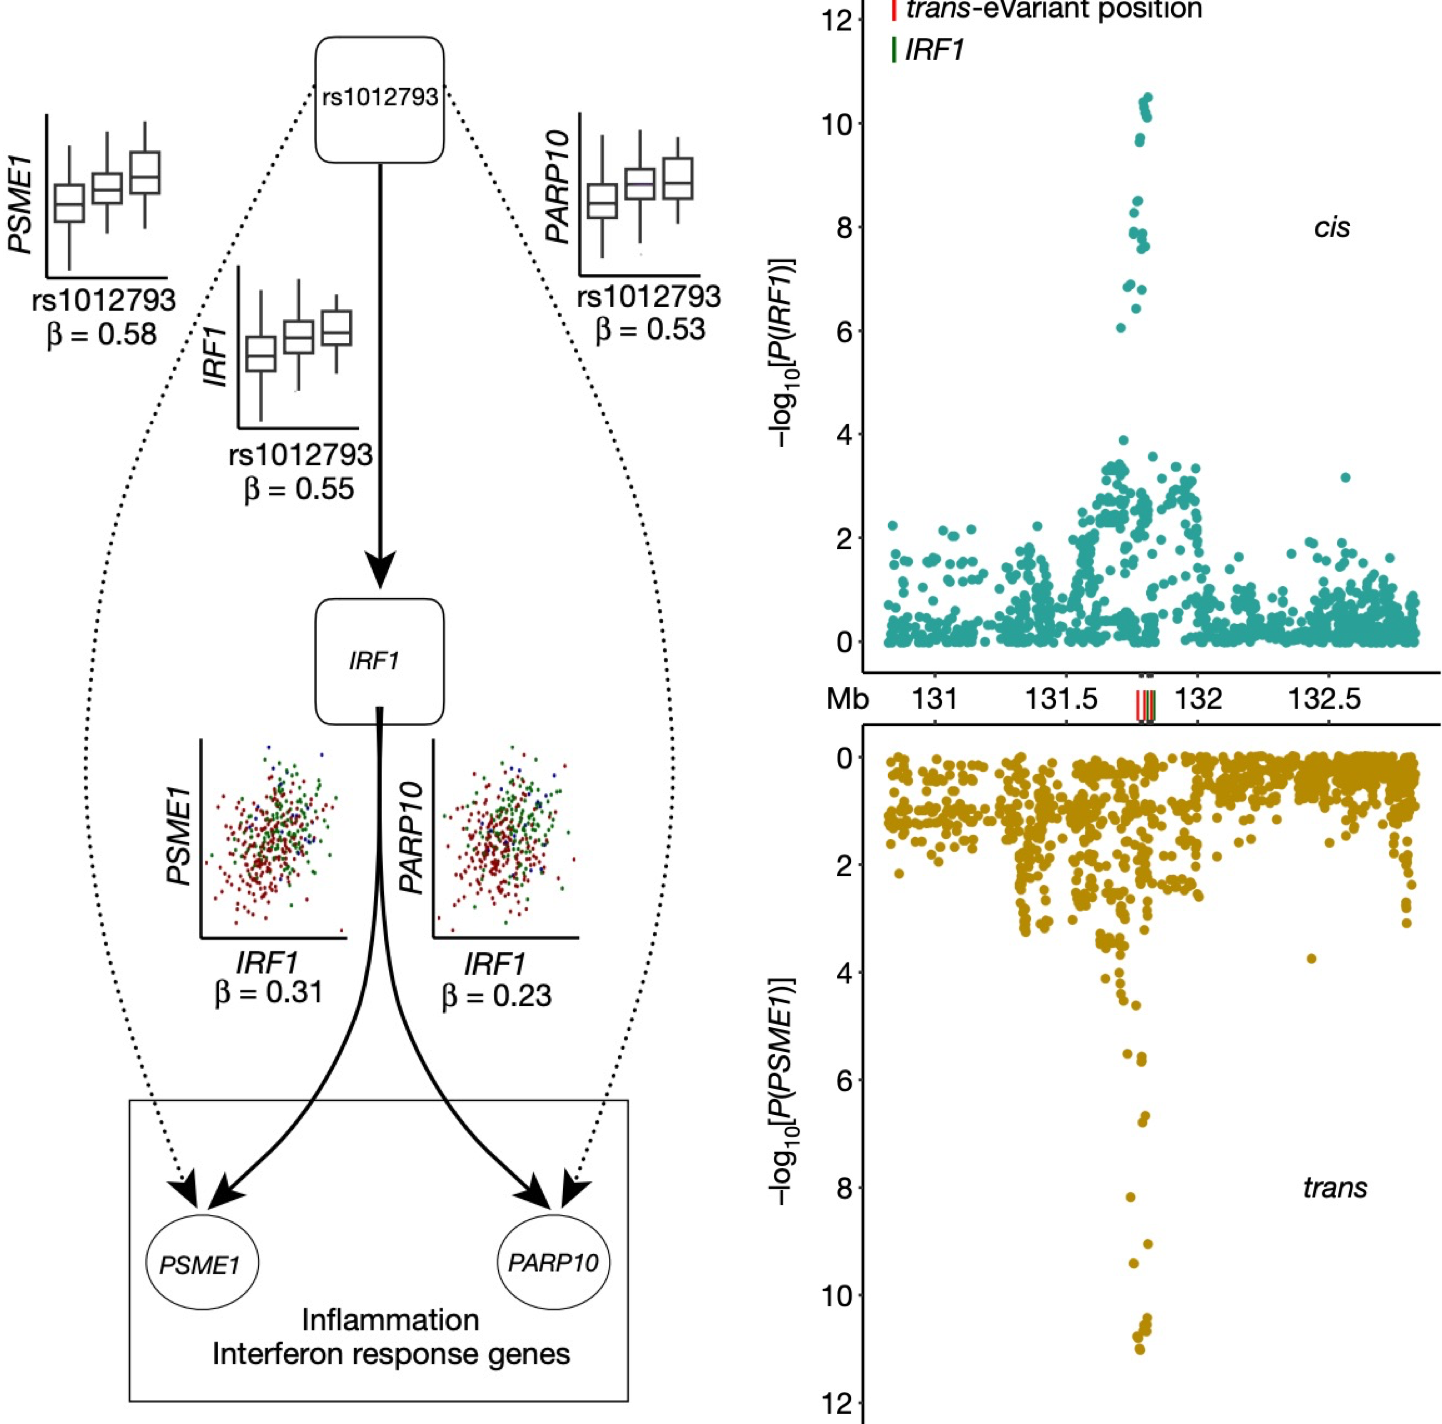
\includegraphics[width=0.7\linewidth]{cistranseqtl}
		\label{fig:cistranseqtl}
	\end{figure}
	\item eg. From GTEx thyroid expression levels\\
	• SNP rs1012793 affects expression of IRF1 in cis and PSME1 and PARP10 in trans
\end{itemize}
\subsection{human vs model organism}
\begin{itemize}
	\item human harder to collect data
	\item model organisms can be cultured in a lab
	\item Yeast recombinant inbred lines, instead of population of unrelated individuals
	\begin{itemize}
		\item two founder strains, BY and RM\\
		– Mate the founders in a lab for generations\\
		– Genotype/expression profile for ~110 progenies\\
		– In a follow-up study\\
		---- The same founders, ~1000 progenies, whole-genome sequencing, RNA-seq
	\end{itemize}
	\item effect of recombination
	\begin{itemize}
		\item schuffle genome through mating
		\item More generations of mating means more shuffling through recombinations and higher resolution for eQTL mapping
	\end{itemize}
\end{itemize}
\subsection{allele-specific eQTL mapping}
\begin{itemize}
	\item cis-acting elements - DNA sequences in the regulatory region of the gene(e.g.,TF binding	sites)
	\item trans-acting elements - RNA and proteins that interact w cis
	\item problem:
	\begin{itemize}
		\item assumed cis = local and trans = distant, but not the case
		\item exists nearby trans and distant cis
	\end{itemize}
	\item fix: \kyw{allele-specifc expression quantification w transcriptome RNA-seq}
	\begin{itemize}
		\item diploid: maternal / paternal allele diff, RNA-seq can capture this
	\end{itemize}
	\item idea: between two species
	\begin{itemize}
		\item Studied cis/trans regulatory divergence between two species
		– First study that makes use of allele-specific gene expressions to learn about gene regulatory network
		– Examines genome / transcriptome data for two parent species and their F1 progeny
	\end{itemize}
	\item idea: extension to population genome / transcriptome data
\end{itemize}

\subsection{allele specific eQTL mapping}
\begin{itemize}
	\item cis-trans regulatory divergence in two species
	\item cis / trans, but location not very helpful
	\item Only cis-regulatory divergence between two species
	\begin{itemize}
		\item only in each chromosomes? local?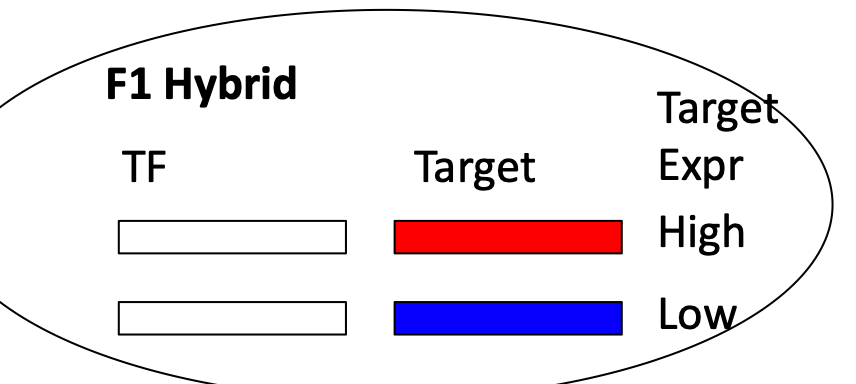
\includegraphics[width=0.5\linewidth]{cis-regulatory}
		\item no cross regulation $\to$ high and low
	\end{itemize}
	\item trans-regulatory divergence:
	\begin{itemize}
		\item 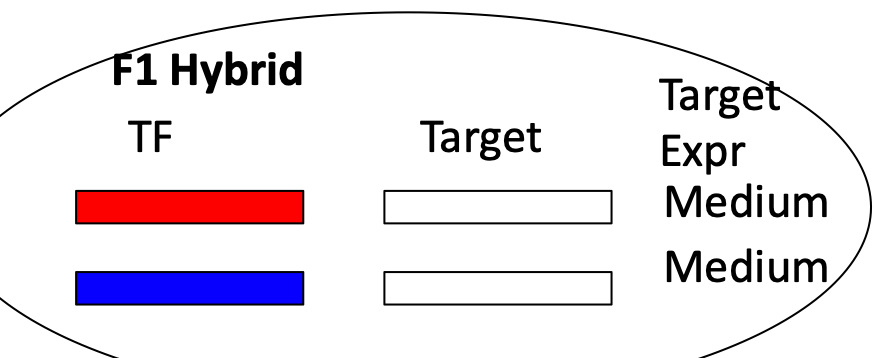
\includegraphics[width=0.5\linewidth]{trans-regulatory}
		\item both are medium $\to$ got averaged out
		\item since there are trans-regulation
		\item one transcription factor is less efficient than the other
	\end{itemize}
	\item ratio between the high and low in parents vs. ratio in F1 progeny
	\item ratio = 1 $\to$ trans-regulatory divergence
	\item $ y = x \to $ cis-regulatory divergence
	\item most genes are influced by a mix of the two
	\item regulatory genes tend to be trans-acting
	\item structural genes: Usually terminal nodes with no trans- acting effects
\end{itemize}

\subsection{limitations}
\begin{itemize}
	\item only examine 2 species and offspring (sample size too small)
	\item can do on population
	\item Population-based study: allele-specific eQTL mapping
	\item Cis-acting eQTLs = cis-regulatory variation
	\begin{itemize}
		\item linear model wrt alleles (eg, A, C, T, G)
	\end{itemize}
	\item Trans-acting eQTLs = trans-regulatory variation
	\begin{itemize}
		\item linear model wrt genotypes (eg, AA, Aa, CG)
	\end{itemize}
\end{itemize}
\newpage
\section{scRNA-seq \& CRISPR}
\subsection{Background}
\begin{itemize}
	\item experimental validation of eQTL w CRISPR perturbation
	\begin{itemize}
		\item genome editing w CRISPR, followed by scRNA
	\end{itemize}
	\item scRNA made possible
	\begin{itemize}
		\item Cell–type specific eQTLs
		\item  Co-expression eQTLs
	\end{itemize}
\end{itemize}

\subsection{co-expression eQTLs}
\begin{itemize}
	\item one vector for expression and one vector for genotype
	\item coexpression eQTL: study eQTLs that influence “co-expression” between two genes
	\item $\to$ personal gene regulatory network
\end{itemize}

\subsection{CRISPR}
\begin{itemize}
	\item genetic screnning
	\item three components
	\begin{itemize}
		\item Perturb:Knockout,RNAi,CRISPR
		\item Model:primary cells,organoids,mice
		\item Assay:measuring phenotypes of interest,RNA-seq,scRNA-seq
	\end{itemize}
	\item Cas9 molecule
	\begin{itemize}
		\item acomponentofthetypeIICRISPR bacterial adaptive immune system
		\item DNAdouble-strandbreak(DSB)by Cas9 is repaired by the endogenous DNA DSB repair pathways
	\end{itemize}
	\item sgRNA (single guide RNA)
	\begin{itemize}
		\item guide Cas9 to the correct place
		\item 20bp complimentary to the target DNA
	\end{itemize}
	\item CRISPR knockout
	\item CRISPR interference
	\begin{itemize}
		\item repress gene of interest
	\end{itemize}
	\item CRISPR activation
	\begin{itemize}
		\item overexpress the gene of interest
	\end{itemize}
\end{itemize}
\subsection{array vs pooled screening}
\begin{itemize}
	\item array screening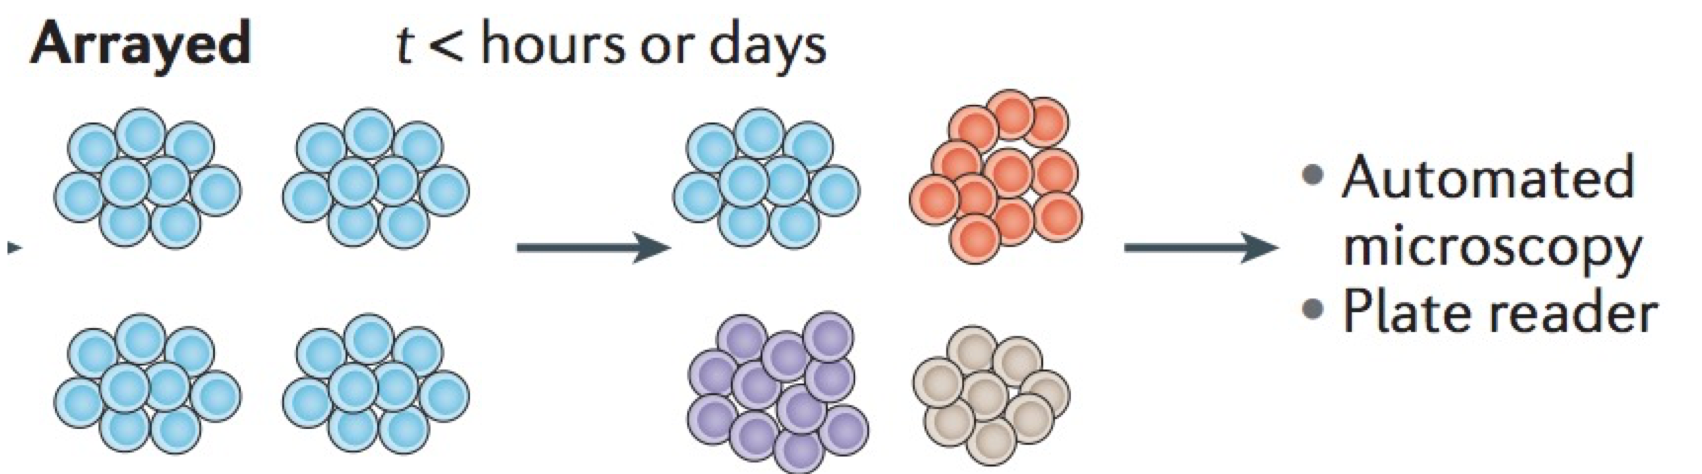
\includegraphics[width=0.7\linewidth]{arrayscreening}
	
	\item pooled screening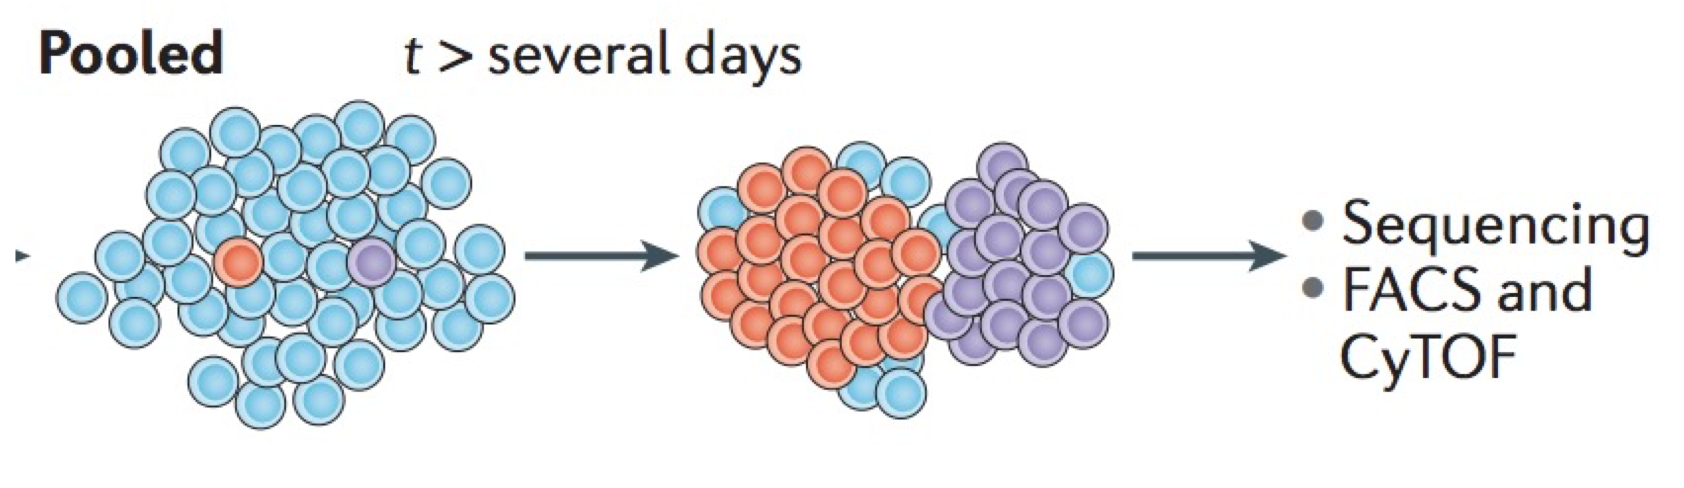
\includegraphics[width=0.7\linewidth]{pooledscreening}
	\item viability screens
	\begin{itemize}
		\item negative screen\\
		Perturbations that reduce cell fitness will be depleted by the end of the screen
		\item positive screen\\
		Perturbations that give survival advantage to the cells, e.g., alternative culture conditions, small molecules
	\end{itemize}
\end{itemize}









\end{document}
